\chapter{Espaces vectoriels}
\origpage{163--200}

\BellaSection{1. Définitions, exemples, premières propriétés}

\medskip\noindent\textsc{Définition 6.1.} --- \emph{On appelle espace vectoriel sur un corps commutatif, $K$, tout ensemble $E$ muni d'une loi de composition interne, l'addition, qui lui donne une structure de groupe abélien, et tel qu'il existe une loi de composition externe, la multiplication par un scalaire, vérifiant
\begin{enumerate}[label=\arabic*),leftmargin=2.1em]
\item $\forall\lambda\in K$, $\forall(X,Y)\in E^2$, $\lambda(X+Y)=\lambda X+\lambda Y$,
\item $\forall(\lambda,\mu)\in K^2$, $\forall X\in E$, $(\lambda+\mu)X=\lambda X+\mu X$,
\item $\forall(\lambda,\mu)\in K^2$, $\forall X\in E$, $\lambda(\mu X)=(\lambda\mu)X$,
\item $\forall X\in E$, $1\cdot X=X$, (1 élément neutre du produit dans $K$).
\end{enumerate}}

\medskip\noindent\textsc{Exemple 6.2.} --- Le corps commutatif $K$, est un espace vectoriel sur lui-même, pour l'addition et le produit existant sur $K$.

Les éléments d'un espace vectoriel $E$ sur $K$ sont appelés vecteurs et ceux du corps $K$ scalaires. Si la loi multiplicative de $K$ n'est pas commutative, on parle de structure de module, qui se définit plus généralement en remplaçant $K$ par un anneau.

\medskip\noindent\textsc{Exemple 6.3.} --- Soit $n\in\mathbb N^*$ un entier non nul, on définit le produit cartésien $K^n$ comme suit.

Si $n=1$, $K^1=K$.

Si $n=2$, $K^2=K\times K$ est l'ensemble des couples formés d'éléments de \BellaCorrectionNote{$K$}{$E$}{Puisque $K^2=K\times K$, ses composantes appartiennent à $K$.}, (voir chapitre 1, §3).

Si $n=3$, \BellaCorrectionNote{$K^3$}{$K=3$}{Il s'agit du produit cartésien de trois copies de $K$.} $=K^2\times K$ par définition, c'est donc l'ensemble des couples du type $(a,z)$ avec $a$ dans $K^2$ donc du type $a=(x,y)$ avec $x$ et $y$ dans $K$. Au lieu de noter $((x,y),z)$ l'élément générique de $K^3$, on le note $(x,y,z)$ et on parle du triplet, $(x,y,z)$ de $K^3$.

Plus généralement, $K^n$ sera, par définition, le produit cartésien de $K^{n-1}$ par $K$, soit $K^n=K^{n-1}\times K$, et par commodité, on notera $(x_1,x_2,\ldots,x_n)$ l'élément générique de $K^n$, (avec chaque $x_i\in K$) appelé $n$-uplet.

Formellement, on définit donc $K^n$ à partir des couples. Sur $K^n$, on définit une structure d'espace vectoriel en posant : pour $X=(x_1,\ldots,x_n)$ et $Y=(y_1,\ldots,y_n)$ dans $K^n$, et $\lambda$ dans $K$,
\[
X+Y=(x_1+y_1,\ldots,x_n+y_n),
\]
\[
\lambda X=(\lambda x_1,\lambda x_2,\ldots,\lambda x_n),
\]
et il est facile de vérifier que l'on a une structure d'espace vectoriel.

\medskip\noindent\textsc{Exemple 6.4.} --- Soient $E_1,\ldots,E_n$, $n$ espaces vectoriels sur le corps commutatif $K$, en procédant par récurrence comme pour $K^n$, on définit le produit cartésien
\[
E=E_1\times E_2\times\cdots\times E_n\quad\text{encore noté}\quad E=\prod_{i=1}^n E_i,
\]
dont les éléments sont les $n$-uplets $X=(X_1,\ldots,X_n)$, avec $\forall i=1\ldots n$, $X_i\in E_i$.

Il est facile de vérifier que pour l'addition $+$ définie par
\[
(X_1,\ldots,X_n)+(Y_1,\ldots,Y_n)=(X_1+Y_1,\ldots,X_i+Y_i,\ldots,X_n+Y_n)
\]
$E$ est un groupe additif, et qu'avec le produit
\[
\lambda X=\lambda(X_1,\ldots,X_n)=(\lambda X_1,\lambda X_2,\ldots,\lambda X_n)
\]
on munit $E$ d'une structure vectorielle.

\medskip\noindent\textsc{Exemple 6.5.} --- Soit un ensemble non vide $A$ et un espace vectoriel $E$ sur le corps $K$. L'ensemble $E^A$ des applications de $A$ dans $E$ est muni d'une structure vectorielle sur $K$ de la manière suivante.

Si $f$ et $g$ sont deux fonctions de $A$ dans $E$, et $\lambda$ un scalaire dans $K$ on définit la fonction $f+g$ par
\[
\forall x\in A,\qquad (f+g)(x)=f(x)+g(x),
\]
et la fonction $\lambda f$ par
\[
\forall x\in A,\qquad (\lambda\cdot f)(x)=\lambda f(x),
\]
et là encore c'est un jeu de vérifier qu'on a une structure vectorielle pour l'espace des applications de $A$ dans l'espace vectoriel $E$.

\subsection*{6.6. Quelques conséquences de la structure vectorielle}

Soit $E$ espace vectoriel sur $K$. On a, $\forall(\lambda,\mu)\in K^2$, $\forall X\in E$,
\[
(\lambda-\mu)X=\lambda X-\mu X
\]
car dans le groupe additif $E$, cette égalité équivaut à $(\lambda-\mu)X+\mu X=\lambda X$, or le 1er membre vaut $[(\lambda-\mu)+\mu]X$ soit $\lambda\cdot X$. \bookend

De même, $\forall\lambda\in K$, $\forall(X,Y)\in E^2$, $\lambda(X-Y)=\lambda X-\lambda Y$ puisque c'est équivalent à $\lambda(X-Y)+\lambda Y=\lambda X$, ce qui est vrai, le premier membre valant $\lambda[(X-Y)+Y]=\lambda X$.

Il résulte de ces 2 règles de calcul, que

\subsection*{6.7.}
\[
\forall X\in E,\quad 0_KX=0_E\qquad\text{et que}\qquad \forall\lambda\in K,\quad \lambda0_E=0_E
\]
($0_K$ scalaire nul dans $K$, $0_E$, vecteur nul dans le groupe additif $E$), ces résultats étant obtenus avec $\lambda=\mu$ ou $X=Y$ dans les calculs précédents. En fait on a le

\medskip\noindent\textsc{Théorème 6.8.} --- \emph{Dans un espace vectoriel $E$ sur un corps commutatif $K$ on a
\[
(\lambda X=0_E)\Longleftrightarrow(\lambda=0_K\ \text{ou}\ X=0_E).
\]}

Le ou n'étant pas exclusif.

Il suffit de justifier l'implication $(\lambda X=0_E)\Rightarrow(\lambda=0_K$ ou $X=0_E)$ vu ce qui précède.

Or si $\lambda X=0_E$ avec $\lambda\ne0_K$, $\lambda^{-1}$ existe dans $K$ donc $\lambda^{-1}(\lambda X)=\lambda^{-1}0_E=0_E$, c'est aussi $(\lambda^{-1}\lambda)X=1X=X$ d'où $\lambda\ne0_K\Rightarrow X=0_E$. \bookend

Désormais, on écrira indifféremment 0 pour $0_E$ ou $0_K$, le contexte justifiant de quel élément nul il s'agit.

De même, on ne précisera plus que le corps est commutatif, ce qui est supposé une fois pour toutes.

\BellaSection{2. Sous-espaces vectoriels}

\medskip\noindent\textsc{Définition 6.9.} --- \emph{On appelle sous-espace vectoriel d'un espace vectoriel $E$ sur le corps $K$, toute partie $F$ de $E$ qui est sous-groupe additif de $E$ et telle que $\forall\lambda\in K$, $\forall X\in F$, $\lambda X\in F$.}

Il est alors évident que $F$ est un espace vectoriel sur $K$, les conditions de la définition 6.1 étant vérifiées.

\medskip\noindent\textsc{Exemple 6.10.} --- $\{0\}$ et $E$ sont sous-espaces vectoriels de $E$.

\medskip\noindent\textsc{Exemple 6.11.} --- Soit $E$ un espace vectoriel, on considère d'abord l'espace vectoriel $E^{\mathbb N}$ des applications de $\mathbb N$ dans $E$.

L'usage fait qu'on appelle suite $u$ de terme général $u_n$ l'application $u$, élément de $E^{\mathbb N}$, en notant $u_n$ au lieu de $u(n)$ la valeur prise par la fonction $u$ lorsque la variable prend la valeur $n$.

Bien sûr, on peut définir des suites à valeurs dans un ensemble $E$ quelconque.

Si $E$ est le corps $K$ lui-même, ($K=\mathbb Q$, $\mathbb R$ ou $\mathbb C\ldots$) on parle généralement de suite numérique.

Soit alors dans l'espace vectoriel $E=K^{\mathbb N}$ des suites numériques sur $K$ le sous-ensemble $F$ des « suites finies », c'est-à-dire des suites $u$ telles qu'il existe un entier $d(u)$ tel que $\forall n>d(u)$, $u_n=0$.

Ou encore, $u$ application de $\mathbb N$ dans $K$, ne prend qu'un nombre fini de valeurs non nulles, ce nombre fini variant avec $u$.

Cet ensemble $F$ est un sous-espace vectoriel de $E$. Pour le vérifier nous allons employer le critère pratique suivant :

\subsection*{6.12. Critère pratique}
Une partie $F$ d'un espace vectoriel $E$ sur $K$ est un sous-espace vectoriel de $E$ si et seulement si
\begin{enumerate}[label=\arabic*),leftmargin=2.1em]
\item $F\ne\varnothing$,
\item $\forall(X,Y)\in F^2$, $\forall(\lambda,\mu)\in K^2$, $\lambda X+\mu Y\in F$.
\end{enumerate}

D'abord si $F$ est sous-espace de $E$, en tant que sous-groupe additif $F$ est non vide car contient 0, élément nul de $E$ ; puis si $X$ et $Y$ sont dans $F$ et $\lambda$ et $\mu$ dans le corps $K$, $\lambda X$ et $\mu Y$ sont dans $F$, (cf. définition 6.9) qui est stable pour l'addition, donc $\lambda X+\mu Y\in F$.

Réciproquement, si 1) et 2) sont vérifiées, avec $\lambda=1$ et $\mu=-1$ et $X$ et $Y$ dans $F$ on a :
\[
(F\ne\varnothing)\quad\text{et}\quad(\forall(X,Y)\in F^2,\ X-Y\in F)
\]
ce qui justifie déjà que $F$ est sous-groupe additif de $E$, (critère 4.5), puis le 2) avec $\mu=0$ donne $(\forall X\in F)(\forall\lambda\in K)(\lambda X\in F)$. On a bien $F$ sous-espace vectoriel de $E$.

Retour au cas des suites finies : $F=\{$suites finies à valeurs dans $K\}$ n'est pas vide, car $u=0$, (telle que, $\forall n\in\mathbb N$, $u_n=0$) est un élément de $F$, puis si $u$ et $v$ sont dans $F$ et $\lambda$ et $\mu$ dans le corps $K$, comme
\[
\forall n>d(u)\quad u_n=0
\]
et
\[
\forall n>d(v)\quad v_n=0,
\]
il est clair que $\forall n>\sup(d(u),d(v))$, (qui est un entier), on a
\[
(\lambda u+\mu v)_n=\lambda u_n+\mu v_n=0
\]
donc la suite $\lambda u+\mu v$ est finie.

\subsection*{6.13.}
En fait, les suites finies à valeurs dans $K$ sont encore appelées polynômes à coefficients dans $K$, si $u$ est un polynôme non nul il existe un entier $d(u)$ tel que le terme $u_{d(u)}$ soit non nul et que $\forall n>d(u)$, $u_n=0$ : cet entier est le degré du polynôme $u$, et au lieu de noter
\[
(u_0,u_1,\ldots,u_{d(u)},0,0,\ldots,0,\ldots)
\]
un polynôme, on le note
\[
u_0+u_1X+u_2X^2+\cdots+u_nX^n,
\]
pour des raisons exposées dans le chapitre 7 sur les polynômes.

On note également :

\subsection*{6.14.}
$K[X]$ l'espace vectoriel des polynômes sur le corps $K$, espace appelé à un riche avenir. Structurellement, c'est l'espace vectoriel des suites finies à valeurs dans $K$.

\subsection*{Sous-espaces vectoriels et intersection}

\medskip\noindent\textsc{Théorème 6.15.} --- \emph{Toute intersection de sous-espaces vectoriels d'un espace vectoriel $E$ est un sous-espace vectoriel de $E$.}

Soit donc $(F_i)_{i\in I}$ une famille de sous-espaces vectoriels de $E$ et
\[
F=\bigcap_{i\in I}F_i.
\]
Si $I=\varnothing$, $F=E$ est un sous-espace vectoriel de $E$. On suppose $I$ non vide.

Comme le vecteur nul, 0, est dans chaque $F_i$, on a $0\in F$ qui est non vide, puis si $(X,Y)\in F^2$ et $(\lambda,\mu)\in K^2$, comme $F\subset F_i$, pour tout $i$ de $I$ et que $F_i$ est sous-espace vectoriel, on a, $\forall i\in I$, $\lambda X+\mu Y\in F_i$, d'où $\lambda X+\mu Y\in F$, donc $F$ est bien sous-espace vectoriel de $E$. \bookend

Comme pour la notion de sous-groupe engendré par une partie, on va introduire le sous-espace vectoriel engendré par une partie, et on aura une approche globale, ou élément par élément, de ce sous-espace.

\medskip\noindent\textsc{Définition 6.16.} --- \emph{Soit $A$ une partie de $E$ espace vectoriel sur $K$. On appelle sous-espace vectoriel engendré par $A$ le plus petit sous-espace vectoriel de $E$ contenant $A$. On le note $\operatorname{Vect}(A)$.}

\medskip\noindent\textsc{Théorème 6.17.} --- \emph{Le sous-espace $\operatorname{Vect}(A)$ est l'intersection de tous les sous-espaces vectoriels de $E$ contenant $A$.}

Car si $\mathcal F=\{F;\ F\text{ sous-espace vectoriel de }E,\ A\subset F\}$ on a $E\in\mathcal F$ qui est donc non vide ; puis
\[
F_0=\bigcap_{F\in\mathcal F}F
\]
est un sous-espace vectoriel de $E$, (théorème 6.15).

De plus $A\subset F_0$, (car contenu dans chaque $F$ dont on prend l'intersection).

Enfin, $F_0$ est bien le plus petit sous-espace vectoriel contenant $A$ car $F_0$ est inclus dans chaque sous-espace vectoriel contenant $A$. Donc $F_0=\operatorname{Vect}(A)$. \bookend

Cette approche globale de $\operatorname{Vect}(A)$ va être précisée en caractérisant les éléments de $\operatorname{Vect}A$. Pour cela, il nous faut parler de combinaison linéaire de vecteurs.

\medskip\noindent\textsc{Définition 6.18.} --- \emph{Soient $X_1,X_2,\ldots,X_n$ des vecteurs de $E$ en nombre fini, $n\in\mathbb N^*$. On appelle combinaison linéaire des $(X_i)_{1\le i\le n}$, tout vecteur du type
\[
X=\lambda_1X_1+\lambda_2X_2+\cdots+\lambda_nX_n=\sum_{i=1}^n\lambda_iX_i,
\]
les $\lambda_i\in K$.}

Au passage, on a introduit le symbole $\sum_{i=1}^n$ de sommation. Il faut bien comprendre qu'il s'agit d'une somme d'un nombre fini de vecteurs.

\medskip\noindent\textsc{Théorème 6.19.} --- \emph{Soit une partie non vide $A$ de $E$ espace vectoriel sur le corps $K$. Alors $\operatorname{Vect}(A)$ est l'ensemble des combinaisons linéaires formées à partir des vecteurs de $A$.}

Si $A=\varnothing$, $\operatorname{Vect}(A)=\{0\}$ et il est difficile de parler de combinaisons linéaires dans ce cas. La notation $\operatorname{Vect}(A)$ est introduite en 6.17.

Par ailleurs, il faut comprendre que, dans la définition 6.18 on n'impose pas aux vecteurs $X_i$ d'être distincts. En fait, on a une famille d'éléments de $E$ indexée par $\{1,2,\ldots,n\}$, segment de $\mathbb N$. On note alors $\widetilde A$ l'ensemble de toutes les combinaisons linéaires formées à partir de toutes les familles d'éléments de $A$ indexées par toutes les parties finies non vides de $\mathbb N$.

On va prouver que $\operatorname{Vect}A=\widetilde A$ en justifiant que $\widetilde A$ est sous-espace vectoriel de $E$, contenant $A$ et contenu dans $\operatorname{Vect}A$. Le côté « plus petit... » de $\operatorname{Vect}(A)$ impliquera l'égalité.

$\widetilde A$ est non vide, car $A$ non vide, et $A\subset\widetilde A$ puisque, si $X\in A$, $X=1X$ est une combinaison linéaire finie d'éléments de $A$.

Si $X$ et $Y$ sont dans $\widetilde A$ et $\lambda$ et $\mu$ dans $K$, il existe deux ensembles finis de $\mathbb N$, $I$ et $J$, tels que
\[
X=\sum_{i\in I}\lambda_iX_i\qquad\text{et}\qquad Y=\sum_{j\in J}\mu_jY_j
\]
les $\lambda_i$ et $\mu_j$ étant dans $K$, les $X_i$ et les $Y_j$ dans $A$.

De plus, on peut imposer à $I$ et $J$ d'être disjoints, quitte à translater les éléments de $J$ de la valeur $n_0=1+\sup(I)$ par exemple.

Alors
\[
\lambda X+\mu Y=\sum_{i\in I}\lambda\lambda_iX_i+\sum_{j\in J}\mu\mu_jY_j
\]
est bien dans $\widetilde A$, en tant que combinaison linéaire d'un nombre fini d'éléments de $A$.

On a donc $\widetilde A$ sous-espace vectoriel de $E$, contenant $A$, d'où forcément $\operatorname{Vect}(A)\subset\widetilde A$ puisque $\operatorname{Vect}(A)$ est le plus petit sous-espace contenant $A$.

Or $\operatorname{Vect}(A)$ est stable par combinaisons linéaires, et $A\subset\operatorname{Vect}(A)$ implique $\widetilde A\subset\operatorname{Vect}(A)$ d'où finalement $\operatorname{Vect}(A)=\widetilde A$. \bookend

\medskip\noindent\textsc{Théorème 6.20.} --- \emph{Soient $F_1,F_2,\ldots,F_n$ des sous-espaces vectoriels de $E$ en nombre fini, $n\ge2$. Alors $\operatorname{Vect}(F_1\cup F_2\cup\cdots\cup F_n)$ est l'ensemble
\[
\{X_1+X_2+\cdots+X_n;\ X_i\in F_i\}
\]
encore noté $F_1+F_2+\cdots+F_n$.}

La démarche va être analogue à celle du théorème 6.19. Soit $A=F_1\cup\cdots\cup F_n$ et $\widetilde A=\{X_1+X_2+\cdots+X_n;\ X_i\in F_i\}$. On va prouver que $\widetilde A$ est sous-espace vectoriel contenant $A$, d'où $\operatorname{Vect}(A)\subset\widetilde A$ ; puis l'inclusion $\widetilde A\subset\operatorname{Vect}A$.

D'abord $0\in\widetilde A$ car 0 est dans chaque $F_i$, d'où $0=0+0+\cdots+0\in\widetilde A$. On a déjà $\widetilde A$ non vide ; puis si $X$ et $Y$ sont dans $\widetilde A$, $\lambda$ et $\mu$ dans $K$, avec $X_1,\ldots,X_n$ et $Y_1,\ldots,Y_n$ tels que, $\forall i\le n$, $X_i\in F_i$ et $Y_i\in F_i$ et
\[
X=\sum_{i=1}^nX_i,\qquad Y=\sum_{i=1}^nY_i
\]
on a
\[
\lambda X+\mu Y=\sum_{i=1}^n(\lambda X_i+\mu Y_i)
\]
avec $\lambda X_i+\mu Y_i\in F_i$, (stable par combinaison linéaire) donc $\lambda X+\mu Y\in\widetilde A$ d'où $\widetilde A$ sous-espace vectoriel de $E$.

Puis $A=F_1\cup\cdots\cup F_n\subset\widetilde A$ car $\forall X_i\in F_i$, $X_i=0+\cdots+0+X_i+0+\cdots+0\in\widetilde A$ (on prend $X_j=0$, $\forall j\ne i$, $j\le n$) d'où $\operatorname{Vect}(A)\subset\widetilde A$ car $\operatorname{Vect}(A)$ est le plus petit sous-espace vectoriel qui contient $A$, et $\widetilde A$ est un sous-espace vectoriel de $E$, contenant $A$.

Enfin, $\widetilde A\subset\operatorname{Vect}A$ puisque $\widetilde A$ est formé de combinaisons linéaires particulières de vecteurs de $A$. Finalement, on a donc $\operatorname{Vect}(A)=\widetilde A$. \bookend

Cette connaissance de la forme de $\operatorname{Vect}(F_1\cup F_2\cup\cdots\cup F_n)$, les $F_i$ étant des sous-espaces vectoriels de $E$, va nous permettre d'aborder l'étude du comportement de la notion de sous-espace vis-à-vis de la réunion.

D'abord on a le

\medskip\noindent\textsc{Théorème 6.21.} --- \emph{Un espace vectoriel $E$ n'est jamais réunion de deux sous-espaces différents de $E$ et de $\{0\}$.}

C'est la transcription du théorème 4.7 valable pour les groupes, car un espace vectoriel est d'abord un groupe additif.

Rappelons-en brièvement la justification, (ce qui peut éviter de tourner les pages). Si $E=F_1\cup F_2$ avec $F_1$ et $F_2$ sous-espaces différents de $E$ et de $\{0\}$, on a $F_1\ne E\Rightarrow\exists X_2\notin F_1$, comme $E=F_1\cup F_2$ c'est que $X_2\in F_2$ ; de même $F_2\ne E\Rightarrow\exists X_1\notin F_2$, donc $X_1\in F_1$. Puis $X_1+X_2\in E=F_1\cup F_2$, par exemple $X_1+X_2\in F_1$. Comme $X_1\in F_1$ et que $F_1$ est un sous-groupe additif, on a $X_2=-X_1+(X_1+X_2)$ dans $F_1$ ce qui est absurde. \bookend

La situation va se compliquer si on aborde la question d'une réunion de plus de deux sous-espaces : le cardinal du corps va intervenir.

\medskip\noindent\textsc{Théorème 6.22.} --- \emph{Soit $E$ un espace vectoriel sur un corps $K$ de cardinal infini, $E$ n'est jamais réunion d'un nombre fini de sous-espaces vectoriels propres, (c'est-à-dire différents de $E$ et de $\{0\}$), non inclus l'un dans l'autre.}

On va prouver, par récurrence sur l'entier $n\ge2$, que $E$ n'est pas réunion de $n$ sous-espaces propres. C'est vrai pour $n=2$, (6.21).

On suppose le résultat vrai pour $n$.

Soient $n+1$ sous-espaces de $E$, distincts, et différents de $E$ et de $\{0\}$, $F_1,F_2,\ldots,F_n,F_{n+1}$.

On les suppose aussi non inclus l'un dans l'autre.

Soit $F=\operatorname{Vect}(F_1\cup\cdots\cup F_n)=F_1+F_2+\cdots+F_n$, (Théorème 6.20), chaque $F_i$ est $\ne\{0\}$ et aussi $\ne F$, (si $\exists i\le n$ avec $F_i=F$, $\forall j\ne i$, $j\le n$, $F_j\subset F_i$ ce qui contredit l'hypothèse). On applique l'hypothèse de récurrence, pour $n$ et les $F_i$ sous-espaces de $F$, on a :
\[
F_1\cup F_2\cup\cdots\cup F_n\subsetneq F_1+F_2+\cdots+F_n=F.
\]
Il existe donc
\[
Y=X_1+X_2+\cdots+X_n\ \text{dans }F,\qquad Y\notin F_1\cup\cdots\cup F_n.
\]
Soit $H=F_1\cup\cdots\cup F_n\cup F_{n+1}$ : on va prouver que $H$ n'est pas un sous-espace vectoriel.

Si $Y\notin F_{n+1}$, on aura les $X_i$ dans $H$, et $Y=\sum_{i=1}^nX_i\notin H$ : $H$ n'est pas stable par combinaison linéaire, donc pas sous-espace vectoriel.

Si $Y\in F_{n+1}$, et si $H$ était sous-espace vectoriel, comme $F_1\not\subset F_{n+1}$ par hypothèse, $\exists X\in F_1$, $X\notin F_{n+1}$, donc, $\forall\lambda\in K^*=K-\{0\}$ on a $\lambda X+Y\notin F_{n+1}$, sinon, comme $Y\in F_{n+1}$, si $\lambda X+Y\in F_{n+1}$ alors $\lambda X$ serait aussi dans $F_{n+1}$ et comme $\lambda\ne0$, $X=\lambda^{-1}(\lambda X)$ serait dans $F_{n+1}$ : exclu ; de même $\lambda X+Y\notin F_1$, sinon, comme $X\in F_1$, $\lambda X\in F_1\Rightarrow Y\in F_1$, exclu car $Y\notin(F_1\cup\cdots\cup F_n)$.

Mais $X$ et $Y$ sont dans $H$, supposé sous-espace vectoriel de $E$, donc $\lambda X+Y$ est dans $H=F_1\cup F_2\cup\cdots\cup F_n\cup F_{n+1}$, sans être dans $F_1\cup F_{n+1}$ ; c'est que, pour chaque $\lambda$ de $K^*$, il existe un indice $i(\lambda)$ avec $2\le i(\lambda)\le n$, tel que $\lambda X+Y\in F_{i(\lambda)}$. Si $\operatorname{card}(K^*)\ge n$ (ce qui est vrai si $K$ est de cardinal infini) il existe deux $\lambda$ distincts donnant le même indice : d'où $\exists i$, avec $2\le i\le n$ et $\lambda$ et $\lambda'$ distincts tels que $\lambda X+Y\in F_i$ et $\lambda'X+Y\in F_i$.

D'où
\[
\lambda'(\lambda X+Y)-\lambda(\lambda'X+Y)=(\lambda'-\lambda)Y\in F_i.
\]
avec $\lambda'-\lambda\ne0$ et $F_i$ sous-espace vectoriel, il en résulte que $Y$ est dans $F_i$, pour un indice $i\le n$, ce qui contredit l'hypothèse $Y\notin F_1\cup F_2\cup\cdots\cup F_i\cup\cdots\cup F_n$.

On a bien justifié qu'une réunion d'un nombre fini de sous-espaces qui ne se contiennent pas mutuellement, n'est pas un sous-espace vectoriel. \bookend

En fait, si $\operatorname{card}(K)=p$, le passage de $n$ à $n+1$ n'est plus possible si $\operatorname{card}(K^*)=p-1\le n-1$, soit $n\ge p$.

On doit donc s'attendre à avoir des réunions de $p+1$ sous-espaces. C'est effectivement le cas.

Par exemple, $K=\mathbb Z/2\mathbb Z$ a 2 éléments, 0 et 1 avec la règle $1+1=0$, $E=K^2$ a 4 éléments $\{(0,0);(1,0);(0,1)\text{ et }(1,1)\}$ or $E$ est réunion de 3 sous-espaces :
\[
F_1=\{(0,0),(1,0)\},\qquad F_2=\{(0,0),(1,1)\},\qquad F_3=\{(0,0),(0,1)\}.
\]

Plus généralement, avec $p$ premier, et $\operatorname{card}(K)=p$, on vérifierait que $E=K^2$ a $p^2-1=(p-1)(p+1)$ éléments non nuls, (c'est-à-dire distincts de $(0,0)$), et que $E$ est réunion de $p+1$ droites vectorielles.

Après ces résultats sur réunion et intersection, une remarque : le complémentaire ensembliste d'un sous-espace vectoriel n'est jamais sous-espace vectoriel, tout simplement parce qu'il ne contient pas le vecteur nul.

\begin{center}
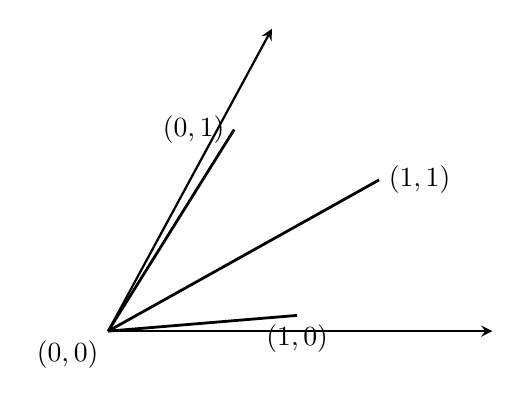
\begin{tikzpicture}[scale=0.80,>=stealth]
\draw[->,line width=0.8pt] (0,0)--(6.1,0);
\draw[->,line width=0.8pt] (0,0)--(2.6,4.8);
\draw[line width=1.0pt] (0,0)--(4.3,2.4);
\draw[line width=1.0pt] (0,0)--(2.0,3.2);
\draw[line width=1.0pt] (0,0)--(3.0,0.25);
\node[below left] at (0,0) {$(0,0)$};
\node[below] at (3.0,0.25) {$(1,0)$};
\node[left] at (2.0,3.2) {$(0,1)$};
\node[right] at (4.3,2.4) {$(1,1)$};
\end{tikzpicture}
\end{center}

\BellaSection{3. Applications linéaires}

\medskip\noindent\textsc{Définition 6.23.} --- \emph{Soient $E$ et $F$ deux espaces vectoriels sur un corps $K$. On appelle application linéaire de $E$ dans $F$ toute application $f$ de $E$ dans $F$ vérifiant :
\begin{enumerate}[label=\arabic*),leftmargin=2.1em]
\item $\forall(X,Y)\in E^2$, $f(X+Y)=f(X)+f(Y)$,
\item $\forall(\lambda,X)\in K\times E$, $f(\lambda\cdot X)=\lambda\cdot f(X)$.
\end{enumerate}}

\medskip\noindent\textsc{Remarque 6.24.} --- On a $f:E\longrightarrow F$ est linéaire si et seulement si
\[
\forall(X,Y)\in E^2,\quad\forall(\lambda,\mu)\in K^2,\quad f(\lambda X+\mu Y)=\lambda f(X)+\mu f(Y).
\]

Cette formulation permet de vérifier la linéarité en un seul calcul. Il est clair que si $f$ est linéaire on a
\begin{align*}
f(\lambda X+\mu Y)&=f(\lambda X)+f(\mu Y),\qquad\text{d'après le 1),}\\
&=\lambda f(X)+\mu f(Y),\qquad\text{d'après le 2) qui traduit le fait que}
\end{align*}
$f$ est un morphisme pour la loi externe.

Réciproquement, si on a la propriété de la remarque, avec $\lambda=\mu=1$ on retrouve le 1) de la définition, et $\mu=0$, $\lambda$ quelconque donne le 2).

\subsection*{6.25. Du vocabulaire}
on parle encore d'homomorphisme d'espace vectoriel au lieu d'application linéaire, d'endomorphisme si $E=F$ ; d'isomorphisme si $f$ est bijective, (et $F$ quelconque) et d'automorphisme lorsque $F=E$ et $f$ bijective.

\medskip\noindent\textsc{Théorème 6.26.} --- \emph{Soient $E$ et $F$ deux espaces vectoriels sur un corps $K$. L'ensemble des applications linéaires de $E$ dans $F$ est un sous-espace vectoriel de l'espace des applications de $E$ dans $F$. On le note $L(E,F)$.}

On a vu, (exemple 6.5), que, $F$ étant un espace vectoriel, l'ensemble $F^E$ des applications de $E$ dans $F$ est muni d'une structure d'espace vectoriel.

On a $L(E,F)\subset F^E$, de plus $L(E,F)$ est non vide, l'application constante nulle, 0, définie par : $(\forall X\in E,\ 0(X)=0_F)$ est linéaire ; et si $f$ et $g$ sont linéaires, si $\alpha$ et $\beta$ sont 2 scalaires, l'application $\alpha f+\beta g$ est linéaire car $\forall(X,Y)\in E^2$, $\forall(\lambda,\mu)\in K^2$, on a
\[
(\alpha f+\beta g)(\lambda X+\mu Y)=\alpha\cdot f(\lambda X+\mu Y)+\beta\cdot g(\lambda X+\mu Y)
\]
\footnote{\textbf{校勘：}原文第一项写作 $f(\lambda X+\lambda Y)$。第二个系数应为 $\mu$，与左端和下一行展开一致。}
par définition des lois sur $F^E$. Or $f$ et $g$ sont linéaires donc on a
\begin{align*}
(\alpha f+\beta g)(\lambda X+\mu Y)
&=\alpha(\lambda f(X)+\mu f(Y))+\beta(\lambda g(X)+\mu g(Y))\\
&=\lambda[\alpha f(X)+\beta g(X)]+\mu[\alpha f(Y)+\beta g(Y)],
\end{align*}
(en utilisant les propriétés de calcul dans l'espace vectoriel $F$), soit encore
\[
(\alpha f+\beta g)(\lambda X+\mu Y)=\lambda((\alpha f+\beta g)(X))+\mu((\alpha f+\beta g)(Y)),
\]
d'où la linéarité de $\alpha f+\beta g$, d'après 6.24.

Donc $L(E,F)$ est non vide, stable par combinaisons linéaires, dans l'espace vectoriel $F^E$ : c'est bien un espace vectoriel. \bookend

\medskip\noindent\textsc{Théorème 6.27.} --- \emph{Soient $E,F,G$ trois espaces vectoriels sur $K$, $f:E\longrightarrow F$ et $g:F\longrightarrow G$ des applications linéaires, alors $g\circ f:E\longrightarrow G$ est linéaire.}

La vérification est immédiate : en enchaînant la linéarité de $f$ puis celle de $g$, on a
\begin{align*}
&\forall(X,Y)\in E^2,\qquad\forall(\lambda,\mu)\in K^2,\\
(g\circ f)(\lambda X+\mu Y)&=g(f(\lambda X+\mu Y))\\
&=g(\lambda f(X)+\mu f(Y))\\
&=\lambda g(f(X))+\mu g(f(Y))\\
&=\lambda(g\circ f)(X)+\mu(g\circ f)(Y).
\end{align*}
\bookend

\medskip\noindent\textsc{Théorème 6.28.} --- \emph{Soient $E$ et $F$ deux espaces vectoriels sur un corps $K$. Si $f$ est un isomorphisme de $E$ sur $F$, son application réciproque $f^{-1}$ en est un de $F$ sur $E$.}

Il s'agit de vérifier la linéarité de $f^{-1}$, qui bien sûr est bijective, comme $f$. Or $\forall(X,Y)\in F^2$, $\forall(\lambda,\mu)\in K^2$, l'égalité
\[
f^{-1}(\lambda X+\mu Y)=\lambda f^{-1}(X)+\mu f^{-1}(Y)
\]
est équivalente à
\[
f[f^{-1}(\lambda X+\mu Y)]=f[\lambda f^{-1}(X)+\mu f^{-1}(Y)]
\]
puisque $f$ est bijective, soit à
\[
\lambda X+\mu Y=\lambda f(f^{-1}(X))+\mu f(f^{-1}(Y))
\]
vu la linéarité de $f$, le second membre est bien $\lambda X+\mu Y$ ce qui achève la justification. \bookend

\medskip\noindent\textsc{Théorème 6.29.} --- \emph{L'ensemble $L(E,E)$ des applications linéaires de $E$ dans $E$ est muni par les lois $+$ et $\circ$ d'une structure d'anneau (non commutatif), par les lois $+$ et produit par un scalaire d'une structure d'espace vectoriel. On le note encore $\operatorname{Hom}(E)$ ou $\operatorname{End}(E)$.}

On appelle encore algèbre un tel ensemble.

Les vérifications sont évidentes. \bookend

\medskip\noindent\textsc{Théorème 6.30.} --- \emph{Soit un espace vectoriel $E$ sur un corps $K$. L'ensemble des automorphismes de $E$ est un groupe (non commutatif) pour le produit de composition. On le note encore $\operatorname{Aut}(E)$ ou, plus souvent $GL(E)$. (Abréviation de groupe linéaire de $E$).}

D'abord $GL(E)$ est non vide car $\operatorname{id}_E:X\longmapsto X$, application identité est linéaire bijective, puis si $f$ est bijective linéaire $f^{-1}$ est aussi linéaire, (Théorème 6.28), enfin si $f$ et $g$ sont linéaires bijectives, $f\circ g^{-1}$ est aussi bijective et linéaire (Théorème 6.27). L'associativité du produit de composition permet de conclure à la structure de groupe. \bookend

\subsection*{Applications linéaires et sous-espaces}

\medskip\noindent\textsc{Théorème 6.31.} --- \emph{Soient $E$ et $F$ deux espaces vectoriels sur un corps $K$ et $f$ une application linéaire de $E$ dans $F$. Si $E'$ est un sous-espace vectoriel de $E$, son image $f(E')$ est un sous-espace vectoriel de $F$. Si $F'$ est un sous-espace vectoriel de $F$, son image réciproque $f^{-1}(F')$ est un sous-espace de $E$.}

Là encore il s'agit de vérifications faciles.

Soit d'abord $E'$ un sous-espace de $E$, il contient le vecteur nul $0_E$, donc $f(E')$ contient $f(0_E)$ or $f$ étant un morphisme de groupe additif en particulier, on a $f(0_E)=0_F$, (voir 4.15), donc $f(E')$ est non vide, puis si $X'$ et $Y'$ sont dans $f(E')$ et $\lambda,\mu$ dans le corps, on a d'abord l'existence de $X$ et $Y$ dans $E'$ tels que $f(X)=X'$ et $f(Y)=Y'$ d'où
\[
\lambda X'+\mu Y'=\lambda f(X)+\mu f(Y)=f(\lambda X+\mu Y)
\]
par linéarité de $f$, or $\lambda X+\mu Y\in E'$ qui est stable par combinaison linéaire en tant que sous-espace de $E$, donc $\lambda X'+\mu Y'\in f(E')$ d'où la stabilité de $f(E')$ par combinaison linéaire : on a bien $f(E')$ sous-espace de $F$.

De manière analogue, $F'$ étant un sous-espace de $F$, on a
\[
f^{-1}(F')=\{X\in E;\ f(X)\in F'\}
\]
qui est non vide car $0_E\in f^{-1}(F')$ puisque $0_F=f(0_E)$ est dans $F'$ ; et $f^{-1}(F')$ est stable par combinaison linéaire car si $X$ et $Y$ sont dans $f^{-1}(F')$, on a $f(X)\in F'$ et $f(Y)\in F'$, d'où, $\forall(\lambda,\mu)\in K^2$, $\lambda f(X)+\mu f(Y)\in F'$, (sous-espace vectoriel de $F$) soit, par linéarité de $f$, $f(\lambda X+\mu Y)\in F'$ ou encore $\lambda X+\mu Y\in f^{-1}(F')$. \bookend

\subsection*{6.32.}
En particulier, si $f\in L(E,F)$, l'image $f(E)$ est sous-espace de \BellaCorrectionNote{$F$}{$E$}{L'image de $f:E\to F$ est une partie de l'espace d'arrivée $F$.} et le noyau de $f$, $\operatorname{Ker}f=f^{-1}(\{0\})=\{X;\ X\in E;\ f(X)=0\}$ est un sous-espace de $E$ et ces sous-espaces particuliers ont un riche avenir devant eux.

\medskip\noindent\textsc{Théorème 6.33.} --- \emph{Soient $E$ et $F$ deux espaces vectoriels sur un corps $K$ et $f$ une application linéaire de $E$ dans $F$. On a
\[
f\text{ injective}\Longleftrightarrow\operatorname{Ker}f=\{0\}.
\]}

Il est inutile de préciser $0_E$ ou $0_F$, le contexte précisant où sont les éléments nuls.

En effet, si $f$ est injective, et si $X\in\operatorname{Ker}f$, on a $f(X)=0=f(0)\Rightarrow X=0$ (injectivité) donc on a bien $\operatorname{Ker}f=\{0\}$ ; et si $\operatorname{Ker}f=\{0\}$, si $f(X)=f(X')$ alors $f(X-X')=f(X)-f(X')=0$ donc $X-X'\in\operatorname{Ker}f$ soit $X-X'=0$, ou encore $X=X'$ d'où l'injectivité. \bookend

Avant d'aborder les espaces vectoriels quotients, notion analogue aux groupes quotients par un sous-groupe distingué, aux anneaux quotients par un idéal bilatère, on peut encore établir des propriétés intéressantes concernant les images et noyaux des $f^p$, puissances de $f$ endomorphisme de $E$.

\subsection*{6.34. Images et noyaux des itérés de $f\in\operatorname{Hom}(E)$}

Soit $E$ un espace vectoriel sur un corps $K$ et $f$ une application linéaire de $E$ dans $E$. On pose $f^0=\operatorname{id}_E$, identité de $E$, et on définit les puissances de $f$ pour le produit de composition, par $f^2=f\circ f$ et $f^{p+1}=f^p\circ f=f\circ f^p$ puisque le produit de composition est associatif.

\medskip\noindent\textsc{Lemme 6.35.} --- \emph{Pour tout $p$ de $\mathbb N$, on a
\[
\operatorname{Ker}f^p\subset\operatorname{Ker}f^{p+1}\qquad\text{et}\qquad \operatorname{Im}(f^p)\supset\operatorname{Im}(f^{p+1}).
\]}

On note $\operatorname{Im}(f)$ l'image $f(E)$, avec $f$ linéaire.

Car si $x\in\operatorname{Ker}f^p$ on a $f^{p+1}(x)=f(f^p(x))=f(0)=0$ donc $x\in\operatorname{Ker}f^{p+1}$ ; et si $y\in\operatorname{Im}f^{p+1}$, il existe $x\in E$ tel que $y=f^{p+1}(x)=f^p(f(x))$ donc $y$ est aussi dans l'image de $f^p$.

Les suites des $\operatorname{Ker}f^p$ et $\operatorname{Im}f^p$ sont donc monotones pour l'inclusion, celle des noyaux est croissante, celle des images est décroissante.

\medskip\noindent\textsc{Lemme 6.36.} --- \emph{S'il existe $p$ tel que $\operatorname{Ker}f^p=\operatorname{Ker}f^{p+1}$, alors $\operatorname{Ker}f^{p+1}=\operatorname{Ker}f^{p+2}$. S'il existe $q$ tel que $\operatorname{Im}f^q=\operatorname{Im}f^{q+1}$, alors $\operatorname{Im}f^{q+1}=\operatorname{Im}f^{q+2}$.}

On suppose que $\operatorname{Ker}f^p=\operatorname{Ker}f^{p+1}$. Comme on a déjà $\operatorname{Ker}f^{p+1}\subset\operatorname{Ker}f^{p+2}$ (lemme 6.35), pour justifier la première partie du lemme, il suffit de justifier l'inclusion $\operatorname{Ker}f^{p+2}\subset\operatorname{Ker}f^{p+1}$, donc de « diminuer d'un cran ». Soit donc $x\in\operatorname{Ker}f^{p+2}$, c'est que $f^{p+2}(x)=f^{p+1}(f(x))=0$, donc que $f(x)\in\operatorname{Ker}f^{p+1}=\operatorname{Ker}f^p$, soit encore que $f^p(f(x))=0$.

On a finalement $f^{p+1}(x)=0$ soit $x\in\operatorname{Ker}f^{p+1}$ et l'inclusion voulue.

Pour le 2e point du lemme, on veut prouver l'égalité $\operatorname{Im}f^{q+1}=\operatorname{Im}f^{q+2}$ or on a déjà l'inclusion $\operatorname{Im}f^{q+2}\subset\operatorname{Im}f^{q+1}$ ; soit donc $y\in\operatorname{Im}f^{q+1}$, il faut « augmenter d'un cran ». On sait qu'il existe $x$ dans $E$ tel que $y=f^{q+1}(x)$. Or augmenter d'un cran s'obtient en traduisant $\operatorname{Im}f^q=\operatorname{Im}f^{q+1}$, on écrit donc que $y=f(f^q(x))$, avec $f^q(x)\in\operatorname{Im}f^q=\operatorname{Im}f^{q+1}$, donc il existe $x'$ dans $E$ tel que $f^q(x)=f^{q+1}(x')$ et finalement $y=f(f^{q+1}(x'))=f^{q+2}(x')$ est bien dans $\operatorname{Im}f^{q+2}$. \bookend

\subsection*{6.37.}
Conséquence du lemme 6.36 : chacune des deux suites monotones est soit strictement monotone, soit strictement monotone jusqu'à un certain rang, puis stationnaire.

En effet, pour les noyaux, on considère $A=\{p;\ p\in\mathbb N,\ \operatorname{Ker}f^p=\operatorname{Ker}f^{p+1}\}$. Si cet ensemble est vide, vu le lemme 6.35, c'est que, pour tout entier $p$, $\operatorname{Ker}f^p\subsetneq\operatorname{Ker}f^{p+1}$ : la suite des noyaux est strictement croissante ; si $A$ n'est pas vide, c'est un ensemble non vide d'entiers, il admet un plus petit élément $p_0$, mais par application itérée du lemme 6.36, on a $\operatorname{Ker}f^{p_0}=\operatorname{Ker}f^{p_0+1}$ donne $\operatorname{Ker}f^{p_0+1}=\operatorname{Ker}f^{p_0+2}$ d'où $\operatorname{Ker}f^{p_0+2}=\operatorname{Ker}f^{p_0+3}\ldots$ et avant $p_0$ il n'y a pas d'égalité, d'où une suite strictement croissante jusqu'au rang $p_0$, puis stationnaire.

On procède de même pour les images.

\subsection*{6.38.}
On peut alors avoir les 4 situations suivantes :
\begin{enumerate}[label=\arabic*),leftmargin=2.1em]
\item aucune des 2 suites ne devient stationnaire ;
\item seule la suite des noyaux devient stationnaire ;
\item seule la suite des images devient stationnaire ;
\item les 2 suites sont stationnaires. Mais alors c'est au même rang.
\end{enumerate}
Les trois premiers points sont du domaine des exemples. L'égalité du 4e point sera justifiée grâce au lemme suivant :

\medskip\noindent\textsc{Lemme 6.39.} --- \emph{Si $\operatorname{Ker}f^k=\operatorname{Ker}f^{k+1}$ et $\operatorname{Im}f^{k+1}=\operatorname{Im}f^{k+2}$ alors $\operatorname{Im}f^k=\operatorname{Im}f^{k+1}$. Si $\operatorname{Im}f^k=\operatorname{Im}f^{k+1}$ et $\operatorname{Ker}f^{k+1}=\operatorname{Ker}f^{k+2}$ alors $\operatorname{Ker}f^k=\operatorname{Ker}f^{k+1}$.}

\textbf{1er point :} on suppose que $\operatorname{Ker}f^k=\operatorname{Ker}f^{k+1}$ et $\operatorname{Im}f^{k+1}=\operatorname{Im}f^{k+2}$. On veut prouver que $\operatorname{Im}f^k=\operatorname{Im}f^{k+1}$ or on sait, (lemme 6.35), que $\operatorname{Im}f^{k+1}\subset\operatorname{Im}f^k$. Il suffit de justifier l'autre inclusion. Soit donc $y=f^k(x)$ un élément de $\operatorname{Im}f^k$, on veut « gagner un cran » ce qui sera possible si on est dans $\operatorname{Im}f^{k+1}$ qui est $\operatorname{Im}f^{k+2}$. Soit donc $f(y)=f^{k+1}(x)\in\operatorname{Im}f^{k+1}=\operatorname{Im}f^{k+2}$ : $\exists x'\in E$ tel que $f(y)=f^{k+1}(x)=f^{k+2}(x')$ d'où, (traduction de l'égalité des noyaux dans sa partie intéressante c'est-à-dire $\operatorname{Ker}f^{k+1}\subset\operatorname{Ker}f^k$),
\[
f^{k+1}(x-f(x'))=0,
\]
(linéarité de $f^{k+1}$), soit $x-f(x')\in\operatorname{Ker}f^{k+1}=\operatorname{Ker}f^k$ : on a $f^k(x-f(x'))=0$ soit encore
\[
y=f^k(x)=f^{k+1}(x')
\]
est bien dans $\operatorname{Im}f^{k+1}$.

\textbf{2e point :} Cette fois il faut prouver que $\operatorname{Ker}f^k=\operatorname{Ker}f^{k+1}$, or $\operatorname{Ker}f^k\subset\operatorname{Ker}f^{k+1}$ est toujours vrai, il reste une inclusion à justifier.

Soit $x$ dans $\operatorname{Ker}f^{k+1}$, il faut « descendre d'un cran », c'est l'égalité $\operatorname{Ker}f^{k+1}=\operatorname{Ker}f^{k+2}$ qui le donnera. On considère donc $y=f^k(x)$, (qui doit être nul), on a $y\in\operatorname{Im}f^k=\operatorname{Im}f^{k+1}$ donc $\exists x'$ tel que $y=f^{k+1}(x')$. Or $f(f^k(x))=f^{k+1}(x)=0$ car $x\in\operatorname{Ker}f^{k+1}$ c'est aussi $=f(f^{k+1}(x'))=f^{k+2}(x')$ donc $x'\in\operatorname{Ker}f^{k+2}$ qui est, par hypothèse, $\operatorname{Ker}f^{k+1}$ : c'est que $y=f^{k+1}(x')=0$, on a finalement justifié l'égalité $f^k(x)=0$.

\subsection*{Conséquence}
On suppose les 2 suites des noyaux et des images stationnaires, avec $r_0$ et $s_0$ entiers tels que
\[
\operatorname{Ker}f^{r_0-1}\subsetneq\operatorname{Ker}f^{r_0}=\operatorname{Ker}f^{r_0+1}=\cdots
\]
et
\[
\operatorname{Im}f^{s_0-1}\supsetneq\operatorname{Im}f^{s_0}=\operatorname{Im}f^{s_0+1}=\cdots
\]
Alors $r_0=s_0$, sinon, par exemple $r_0<s_0$, mais alors on aurait $\operatorname{Ker}f^{s_0-1}=\operatorname{Ker}f^{s_0}$, (car $s_0-1\ge r_0$ : il y a égalité pour les noyaux), et $\operatorname{Im}f^{s_0}=\operatorname{Im}f^{s_0+1}$, le lemme 6.39 implique $\operatorname{Im}f^{s_0-1}=\operatorname{Im}f^{s_0}$ ce qui est exclu.

L'hypothèse $s_0<r_0$ est également absurde, d'où l'égalité. \bookend

\subsection*{Exemples des 4 situations}
On considère l'espace vectoriel $E=K[X]$ des polynômes sur un corps $K$ (6.14). En utilisant les propriétés des bases (Théorème 6.77) on va caractériser $f\in\operatorname{Hom}(E)$ par la donnée des images des vecteurs $(X^p)_{p\in\mathbb N}$ de la base canonique de $E$.

\textit{Exemple 1 :} $f=\operatorname{id}_E$, ($X^p\longmapsto X^p$, $\forall p\in\mathbb N$) : les suites sont stationnaires dès le rang 0.

\textit{Exemple 2 :} dérivation $f$ définie par
\[
X^0=1\longmapsto0,
\]
\[
X\longmapsto1,
\]
\[
\vdots
\]
\[
X^p\longmapsto pX^{p-1},
\]
on vérifie que $f$ est surjective car l'image d'une base est une famille génératrice, (Théorème 6.77), donc, $\forall k$, $\operatorname{Im}f^k=E$, la suite des images est stationnaire, mais il est facile de vérifier que :
\[
\operatorname{Ker}f^0=\{0\},\quad \operatorname{Ker}f=\{\text{polynômes constants}\}
\]
puis
\[
\operatorname{Ker}f^2=\{\text{polynômes 1er degré}\},\ldots,\quad \operatorname{Ker}f^{k+1}=\{\text{polynômes de degré }\le k\}
\]
: il y a inclusions strictes pour les noyaux.

\textit{Exemple 3 :} intégration. Cette fois $f$ est définie par
\[
X^k\longmapsto X^{k+1},
\]
et ce, $\forall k\in\mathbb N$. Alors $f$ est injective, (une base a pour image une famille libre) donc $\forall k$, $\operatorname{Ker}f^k=\{0\}$ : la suite des noyaux est stationnaire, mais pour les images il y a inclusions strictes, car on vérifie que
\[
\operatorname{Im}f^{k+1}=\{\text{polynômes sans termes de degré }0,1,2,\ldots,k\}
\]
contenu strictement dans
\[
\operatorname{Im}f^k=\{\text{polynômes sans termes de degré }0,1,2,\ldots,k-1\}.
\]

\textit{4e cas :} On mélange en définissant $f$ par une « dérivation » sur les indices pairs, et une « intégration » sur les impairs. Disons
\[
X^0\longmapsto0;\qquad \forall n\ge1,\quad X^{2n}\longmapsto X^{2n-2}
\]
et
\[
\forall n\in\mathbb N,\qquad X^{2n+1}\longmapsto X^{2n+3}.
\]
Alors, $\forall n$, $X^{2n+1}=f^n(X)\in\operatorname{Im}f^n$ mais $\notin\operatorname{Im}f^{n+1}$ (si on a un polynôme $P$ tel que $X^{2n+1}=f^{n+1}(P)$, le terme de plus bas degré impair de $f^{n+1}(P)$ est forcément de degré $\ge1+2(n+1)=2n+3$).

Donc il y a inclusions strictes des images, quant aux noyaux, on a $X^{2n}\in\operatorname{Ker}f^{n+1}$ mais $X^{2n}\notin\operatorname{Ker}f^n$ car $f^n(X^{2n})=X^0=1$ d'où inclusions strictes aussi des noyaux.

Enfin signalons qu'en dimension finie, les deux suites sont forcément stationnaires, puisque les dimensions des sous-espaces sont majorées par la dimension de l'espace. (Voir §6 pour les dimensions).

\BellaSection{4. Espace vectoriel quotient, théorèmes d'isomorphisme}

Soit $F$ un sous-espace vectoriel de l'espace vectoriel $E$ sur le corps $K$. C'est en particulier un sous-groupe additif du groupe additif $E$, commutatif, donc $F$ est sous-groupe distingué donc l'ensemble quotient $E/F$ associé à la relation d'équivalence $\mathcal R$ définie par
\[
X\mathcal RY\Longleftrightarrow X-Y\in F
\]
est un groupe additif pour la loi $+$ définie par $\mathcal X+\mathcal Y=$ classe$(X+Y)$ si $X\in\mathcal X$ et $Y\in\mathcal Y$. (Théorème 4.22).

En fait l'équivalence $\mathcal R$ est aussi compatible avec la loi externe : si $X\mathcal RY$, et si $\lambda\in K$, on a $\lambda X\mathcal R\lambda Y$ car $\lambda X-\lambda Y=\lambda(X-Y)$ avec $X-Y\in F$, sous-espace vectoriel, donc $\lambda\cdot(X-Y)\in F$.

En définissant une loi externe sur $E/F$ par $\lambda\mathcal X=$ classe d'équivalence de $\lambda X$, (si $X$ représente $\mathcal X$) ceci a un sens, (indépendance par rapport au choix de $X$ dans $\mathcal X$) et on vérifie les conditions de la définition 6.1.

Par exemple :
\begin{align*}
\lambda(\mathcal X+\mathcal Y)
&=\lambda(\text{classe de }(X+Y))\quad\text{si }X\in\mathcal X\text{ et }Y\in\mathcal Y\\
&=\text{classe }(\lambda(X+Y))\qquad\text{(définition du produit)}\\
&=\text{classe }(\lambda X+\lambda Y),\qquad\text{(calcul dans $E$)}\\
&=\text{classe }\lambda X+\text{classe }\lambda Y,\qquad\text{(somme dans $E/F$)}\\
&=\lambda\,\text{classe}(X)+\lambda\,\text{classe}(Y)\\
&=\lambda\mathcal X+\lambda\mathcal Y.
\end{align*}

On vient de justifier le

\medskip\noindent\textsc{Théorème 6.40.} --- \emph{Soit $F$ un sous-espace vectoriel de l'espace vectoriel $E$ sur le corps $K$. L'ensemble quotient $E/F$ est muni d'une structure vectorielle par les lois :
\[
\mathcal X+\mathcal Y=\operatorname{classe}(X+Y)\qquad\text{et}\qquad \lambda\cdot\mathcal X=\operatorname{classe}(\lambda X)
\]
si $X\in\mathcal X$ et $Y\in\mathcal Y$.}

Il est bon de se rappeler que $\mathcal X$, classe de $X$ est l'ensemble des vecteurs $X+Y$, $Y\in F$, encore noté $\{X\}+F$, (c'est aussi ce qu'on appelle le sous-espace affine de direction $F$ passant par $X$). On peut alors établir deux théorèmes d'isomorphismes, très utiles.

\medskip\noindent\textsc{Théorème 6.41.} --- \emph{(Premier théorème d'isomorphisme) Soient $E$ et $F$ deux espaces vectoriels sur un corps $K$ et $f$ une application linéaire de $E$ dans $F$. On a $E/\operatorname{Ker}f$ isomorphe à $f(E)$.}

En effet, si $X$ et $X'$ sont deux représentants d'une classe $\mathcal X$ élément de $E/\operatorname{Ker}f$, c'est que $X-X'$ est dans $\operatorname{Ker}f$, donc que $f(X-X')=0$ soit $f(X)=f(X')$ par linéarité de $f$. On peut donc définir une application $\varphi$ de $E/\operatorname{Ker}f$ dans le sous-espace $f(E)$ de $F$ en posant $\varphi(\mathcal X)=f(X)$, avec $X\in\mathcal X$, puisque c'est indépendant du choix de $X$ dans $\mathcal X$.

L'application $\varphi$ est linéaire : $\forall(\mathcal X,\mathcal Y)\in(E/\operatorname{Ker}f)^2$, $\forall(\lambda,\mu)\in K^2$, avec $X$ dans $\mathcal X$ et $Y$ dans $\mathcal Y$, on a $\lambda X+\mu Y$ qui représente $\lambda\mathcal X+\mu\mathcal Y$, donc
\begin{align*}
\varphi(\lambda\mathcal X+\mu\mathcal Y)&=f(\lambda X+\mu Y)\\
&=\lambda f(X)+\mu f(Y),\qquad(f\text{ est linéaire}),\\
&=\lambda\varphi(\mathcal X)+\mu\varphi(\mathcal Y)
\end{align*}
d'où la linéarité de $\varphi$.

$\varphi$ est bijective :

-- injective car si $\varphi(\mathcal X)=0$, c'est qu'avec $X$ dans $\mathcal X$ on a $f(X)=0$, soit $X\in\operatorname{Ker}f$ qui est l'élément nul de l'espace quotient $E/\operatorname{Ker}f$, d'où $\mathcal X=0$ ;

-- surjective : soit $Y$ dans le sous-espace $f(E)$ de $F$, on est dans l'image de $f$ donc il existe $X$ dans $E$ tel que $f(X)=Y$ d'où $\varphi(\operatorname{classe}X)=Y$. \bookend

On peut enfin remarquer que, si $s$ est la surjection canonique de $E$ sur $E/\operatorname{Ker}f$, qui à un vecteur $X$ de $E$ associe sa classe $\mathcal X$ dans $E/\operatorname{Ker}f$, et $i$ l'injection canonique de $f(E)$ dans \BellaCorrectionNote{$F$}{$E$}{L'injection canonique considérée est $i:f(E)\hookrightarrow F$, comme l'indique d'ailleurs la formule suivante et le diagramme.} définie par :
\[
\forall Y\in f(E),\qquad i(Y)=Y,\qquad(\text{considéré ici dans }F),
\]
on a $s$ et $i$ linéaires (vérifications évidentes) et $f=i\circ\varphi\circ s$.

\subsection*{6.42. Le diagramme}
\begin{center}
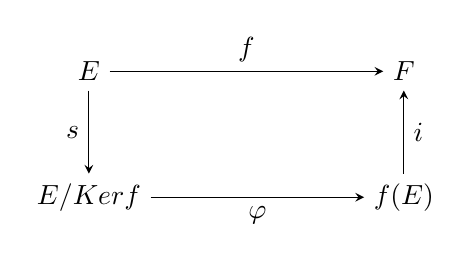
\begin{tikzpicture}[>=stealth]
\node (E) at (0,1.6) {$E$};
\node (F) at (4.0,1.6) {$F$};
\node (Q) at (0,0) {$E/\operatorname{Ker}f$};
\node (I) at (4.0,0) {$f(E)$};
\draw[->] (E)--node[above] {$f$} (F);
\draw[->] (E)--node[left] {$s$} (Q);
\draw[->] (Q)--node[below] {$\varphi$} (I);
\draw[->] (I)--node[right] {$i$} (F);
\end{tikzpicture}
\end{center}
est commutatif.

C'est ce qu'on appelle la décomposition canonique d'une application linéaire. En effet si $X\in E$, et si $\mathcal X=s(X)$ est sa classe d'équivalence on a $\varphi(s(X))=f(X)$, considéré dans l'image de $f(E)$, on l'injecte dans $F$ ce qui donne bien $i\circ\varphi\circ s(X)=i(f(X))=f(X)$ dans $F$ cette fois. \bookend

Voyons maintenant le deuxième théorème d'isomorphisme.

\medskip\noindent\textsc{Théorème 6.43.} --- \emph{Soient $F$ et $G$ deux sous-espaces vectoriels de l'espace $E$ sur le corps $K$. On a
\[
(F+G)/F\simeq G/(F\cap G).
\]
On note $\simeq$ pour isomorphe. On a aussi
\[
(F+G)/G\simeq F/(F\cap G).
\]}

Rappelons que $F+G$ est le sous-espace de $E$ engendré par $F\cup G$, c'est l'ensemble des $X+Y$, $X$ étant dans $F$ et $Y$ dans $G$. On a $F$ sous-espace de $\operatorname{Vect}(F\cup G)$, donc l'espace quotient $(F+G)/F$ existe.

Soit $\mathcal A$ un élément de cet espace quotient, représenté par $A=X+Y$ avec $X\in F$, $Y\in G$ ou par $A'=X'+Y'$ avec $X'\in F$ et $Y'\in G$. On a alors $A-A'=(X-X')+(Y-Y')\in F$, et comme $X-X'\in F$ c'est équivalent à la condition $Y-Y'\in F$, ou encore comme il s'agit de vecteurs du sous-espace vectoriel $G$ de $E$, à la condition $Y-Y'\in F\cap G$. Donc, avec les notations précédentes, si $X+Y$ et $X'+Y'$ représentent le même élément $\mathcal A$ de $(F+G)/F$, on a $Y-Y'\in F\cap G$, soit encore $Y$ et $Y'$ représentent la même classe $\mathcal Y$ de $G/(F\cap G)$.

On pose alors : $\varphi(\mathcal A)=$ classe de $Y$ dans $G/(F\cap G)$, avec $Y$ dans $G$, tel qu'il existe $X$ dans $F$ avec $X+Y$ dans $\mathcal A$.

Il reste à vérifier que $\varphi$ est un isomorphisme de $(F+G)/F$ sur $G/(F\cap G)$.

D'abord $\varphi$ est linéaire : car si $\mathcal A$ et $\mathcal B$ sont deux vecteurs de $(F+G)/F$ représentés par $X+Y$ et $U+V$ avec $X$ et $U$ dans $F$, $Y$ et $V$ dans $G$, et si $\lambda$ et $\mu$ sont 2 scalaires, le vecteur $\lambda\mathcal A+\mu\mathcal B$ admet pour représentant particulier
\[
\lambda(X+Y)+\mu(U+V)=(\lambda X+\mu U)+(\lambda Y+\mu V)
\]
vu la définition des lois sur l'espace quotient.

Donc
\begin{align*}
\varphi(\lambda\mathcal A+\mu\mathcal B)
&=\text{classe de }(\lambda Y+\mu V)\text{ dans }G/(F\cap G)\\
&=\lambda(\text{classe de }Y)+\mu(\text{classe de }V),\qquad(\text{structure quotient}),\\
&=\lambda\varphi(\mathcal A)+\mu\varphi(\mathcal B)\quad\text{par définition de }\varphi.
\end{align*}

$\varphi$ est injective : si $\varphi(\mathcal A)=0$, élément nul de $G/(F\cap G)$, c'est que, si $X+Y$ représente $\mathcal A$, avec $X$ dans $F$ et $Y$ dans $G$, on a $Y$ dans $F\cap G$, donc dans $F$, d'où $X+Y\in F$ et alors $\mathcal A=$ classe (d'un élément de $F$) est l'élément nul de $(F+G)/F$.

Donc $\varphi(\mathcal A)=0\Rightarrow\mathcal A=0$ : on a bien $\varphi$ injective.

$\varphi$ surjective : soit $\mathcal Y$ un élément de $G/(F\cap G)$ de représentant $Y$ dans $G$, si $\mathcal A$ est la classe de $0+Y$ dans $(F+G)/F$, on a bien $\varphi(\mathcal A)=\mathcal Y$ d'où la surjectivité. \bookend

Les deux théorèmes d'isomorphismes fourniront dans les espaces vectoriels de dimension finie, deux formules bien utiles.

\BellaSection{5. Sommes directes}

Soient $F$ et $G$ deux sous-espaces vectoriels d'un espace $E$ sur $K$. On a vu, (Théorème 6.20) que
\[
\operatorname{Vect}(F\cup G)=F+G=\{X+Y;\ X\in F,\ Y\in G\}.
\]

Mais en général, la décomposition d'un vecteur de $F+G$ sous la forme $X+Y$ n'est pas unique. On veut savoir quand il y a unicité. Pour cela on a le

\medskip\noindent\textsc{Théorème 6.44.} --- \emph{Soient $F$ et $G$ deux sous-espaces d'un espace vectoriel $E$. Il y a équivalence entre les conditions
\begin{enumerate}[label=\arabic*),leftmargin=2.1em]
\item $F\cap G=\{0\}$,
\item tout vecteur de $F+G$ s'écrit de manière unique sous la forme $X+Y$ avec $X$ dans $F$ et $Y$ dans $G$.
\end{enumerate}}

1) $\Rightarrow$ 2) car si $Z$ de $F+G$ s'écrit $X+Y$ et $X'+Y'$, l'égalité $X+Y=X'+Y'\Longleftrightarrow X-X'=Y'-Y$ d'où $X-X'\in F\cap G=\{0\}$ donc $X=X'$, et alors $Y=Y'$.

2) $\Rightarrow$ 1) car si $A\in F\cap G$, $-A$ aussi et alors $0=A+(-A)$ avec $A$ dans $F$ et $-A$ dans $G$. Comme on a aussi $0=0+0$, (c'est beau!) avec 0 dans $F$ et 0 dans $G$, (c'est reposant) on a $A=0$ (et pour faire bonne mesure, $-A=0$ ce qui n'ajoute rien au résultat). \bookend

\medskip\noindent\textsc{Définition 6.45.} --- \emph{On dit que $F$ et $G$, sous-espaces de $E$, sont en somme directe si et seulement si $F\cap G=\{0\}$.}

Dans ce cas, on note $F\oplus G$ au lieu de $F+G$, le sous-espace $\operatorname{Vect}(F\cup G)$.

\medskip\noindent\textsc{Définition 6.46.} --- \emph{Deux sous-espaces $F$ et $G$ sont dits supplémentaires si et seulement si $F\oplus G=E$.}

Ou encore
\[
\Longleftrightarrow\quad F\cap G=\{0\}\quad\text{et}\quad F+G=E,
\]
ou
\[
\Longleftrightarrow\quad \forall Z\in E,\ \exists!(X,Y)\in F\times G,\ Z=X+Y,
\]
($\exists!$ signifie il existe un seul, rappelons-le).

\BellaCorrectionNote{Mise en garde}{Mis en garde}{Accord usuel du nom féminin « mise » dans la locution « mise en garde ».} : le fait que $F$ et $G$ soient supplémentaires dans $E$ ne signifie pas que si un vecteur $Z$ n'est pas dans $F$, il est dans $G$; cela signifie que si $Z\notin F$, la composante de $Z$ dans $G$ n'est pas nulle, un point c'est tout! Donc ne pas confondre supplémentaire et complémentaire ensembliste.

Soit alors $F$ et $G$ deux sous-espaces supplémentaires de $E$, l'écriture unique d'un $Z$ de $E$ en $Z=X+Y$ avec $X\in F$ et $Y\in G$ permet de définir deux applications; l'une $p$, de $E$ dans $F$, qui à $Z$ associe $p(Z)=X=$ la composante de $Z$ dans $F$, l'autre, $q$, de $E$ dans $G$ qui à $Z$ associe $q(Z)=Y=$ la composante de $Z$ dans $G$.

Ces applications sont linéaires car si on a aussi $Z'=X'+Y'$ avec $X'\in F$, $Y'\in G$, alors $\forall(\lambda,\lambda')\in K^2$, le vecteur $\lambda Z+\lambda'Z'$ de $E$ se décompose en
\[
\lambda Z+\lambda'Z'=(\lambda X+\lambda'X')+(\lambda Y+\lambda'Y')
\]
avec $\lambda X+\lambda'X'$ dans $F$ et $\lambda Y+\lambda'Y'$ dans $G$, d'où :
\[
p(\lambda Z+\lambda'Z')=\lambda X+\lambda'X'=\lambda p(Z)+\lambda'p(Z'),
\]
de même
\[
q(\lambda Z+\lambda'Z')=\lambda Y+\lambda'Y'=\lambda q(Z)+\lambda'q(Z').
\]

De plus on a $p\circ p=p$ et $q\circ q=q$, car, pour $X$ de $F$, la décomposition dans la somme directe $F\oplus G$ est $X=X+0$ donc $p(X)=X$ mais avec $Z=X+Y$ comme précédemment, on a
\[
p^2(Z)=p(p(Z))=p(X)=X=p(Z),\qquad\text{d'où }p^2=p,
\]
$Z$ étant quelconque dans $E$, et de même $q^2=q$.

Enfin $\operatorname{Im}p=F$, $\operatorname{Ker}p=G$, et $\operatorname{Im}q=G$, $\operatorname{Ker}q=F$. On a déjà $p(Z)=X\in F$, et $\forall X\in F$, $p(X)=X$ donc $\operatorname{Im}p=F$, puis
\[
Z=X+Y\in\operatorname{Ker}p\Longleftrightarrow p(Z)=X=0\Longleftrightarrow Z=Y\in G
\]
d'où $\operatorname{Ker}p=G$. On procède de même pour $q$.

\medskip\noindent\textsc{Définition 6.47.} --- \emph{On appelle projecteur de l'espace vectoriel $E$, toute application linéaire $p$ vérifiant $p\circ p=p$.}

On a donc :

\medskip\noindent\textsc{Théorème 6.48.} --- \emph{Si $E=F\oplus G$ est décomposé en somme directe de deux sous-espaces, l'application qui à $Z$ décomposé en $X+Y$ avec $X$ dans $F$ et $Y$ dans $G$ associe sa composante $X$ dans $F$ est un projecteur d'image $F$ de noyau $G$.}

En fait si $p$ est un projecteur, on a réciproquement une somme directe $E=\operatorname{Ker}p\oplus\operatorname{Im}p$, car, pour tout $Z$ de $E$ on a $p(p(Z))=p(Z)$ soit $p(p(Z)-Z)=0$ par linéarité de $p$ ou encore $Z-p(Z)\in\operatorname{Ker}p$.

Mais alors $Z$ s'écrit $Z=p(Z)+Z-p(Z)$, avec $p(Z)$ dans $\operatorname{Im}p$ et $Z-p(Z)$ dans $\operatorname{Ker}p$, ce qui donne déjà
\[
E=\operatorname{Im}p+\operatorname{Ker}p.
\]
La somme est directe : si $X\in\operatorname{Im}p\cap\operatorname{Ker}p$, il existe un vecteur $T$ tel que $X=p(T)$, puis $p(X)=0$, ($X$ dans le noyau de $p$), soit $p^2(T)=0$. Comme $p^2=p$, il reste $X=p(T)=0$, d'où $\operatorname{Im}p\cap\operatorname{Ker}p=\{0\}$. On vient de justifier le

\medskip\noindent\textsc{Théorème 6.49.} --- \emph{Si $p$ est un projecteur de l'espace vectoriel $E$, on a
\[
E=\operatorname{Ker}p\oplus\operatorname{Im}p.
\]}

\medskip\noindent\textsc{Corollaire 6.50.} --- \emph{Soient $F$ et $G$ deux espaces supplémentaires de $E$, on a $E/F\simeq G$, et $E/G\simeq F$.}

Car avec $p$ projecteur sur $G$, de noyau $F$, (définie, si $Z=X+Y$ avec $X\in F$ et $Y\in G$, par $p(Z)=Y$), le premier théorème d'isomorphisme (Théorème 6.41) s'applique et donne $E/\operatorname{Ker}p\simeq\operatorname{Im}p$, soit $E/F\simeq G$. On procède de même avec le projecteur d'image $F$ et de noyau $G$.

\subsection*{Généralisation des sommes directes\\au cas de plus de deux sous-espaces}

\medskip\noindent\textsc{Théorème 6.51.} --- \emph{Soient $F_1,F_2,\ldots,F_n$ des sous-espaces d'un espace vectoriel $E$ sur un corps $K$, avec $n\ge2$. Les conditions suivantes sont équivalentes :
\begin{enumerate}[label=\arabic*),leftmargin=2.1em]
\item $E=F_1+\cdots+F_n$ et, $\forall i=1,\ldots,n$,
\[
F_i\cap\left(\sum_{\substack{j=1\\j\ne i}}^nF_j\right)=\{0\};
\]
\item tout vecteur de $E$ s'écrit de manière unique sous la forme $X=X_1+\cdots+X_n$ avec, $\forall i=1,\ldots,n$, $X_i\in F_i$;
\item $E=F_1+\cdots+F_n$ et si, avec des $X_i\in F_i$ on a $X_1+\cdots+X_n=0$, chaque $X_i=0$.
\end{enumerate}}

1) $\Rightarrow$ 2) car, chaque $X$ de $E$ est dans $F_1+\cdots+F_n$, donc il existe des $X_i$ dans les $F_i$ tels que $X=X_1+\cdots+X_n$, et si on a une autre décomposition du même $X$ : $X=X'_1+\cdots+X'_n$, avec les $X'_j\in F_j$ aussi alors, $\forall i=1,\ldots,n$, on a
\[
X_i-X'_i=\sum_{\substack{j=1\\j\ne i}}^n(X'_j-X_j)
\]
vu les règles de calcul dans le groupe $E$, d'où
\[
X_i-X'_i\in F_i\cap\left(\sum_{\substack{j=1\\j\ne i}}^nF_j\right)
\]
qui est réduit à $\{0\}$ par hypothèse donc $X_i=X'_i$ et ce, pour chaque $i$ : il y a bien unicité de la décomposition.

2) $\Rightarrow$ 3) Comme tout $X$ de $E$ admet une décomposition en $X=X_1+\cdots+X_n$ avec les $X_j\in F_j$ on a bien $E=\sum_{i=1}^nF_i$ ; et si $X_1+X_2+\cdots+X_n=0$ avec, $\forall i=1,\ldots,n$, $X_i\in F_i$, comme 0 s'écrit aussi $0+0+\cdots+0=0$, puisque 0 est dans chaque sous-espace $F_i$, l'unicité de l'écriture implique que pour chaque $i$, $X_i=0$ d'où le 3).

Enfin 3) $\Rightarrow$ 1) car si on a un vecteur
\[
X\in F_i\cap\sum_{\substack{j=1\\j\ne i}}^nF_j,
\]
ce vecteur $X$ s'écrit sous la forme
\[
X=\sum_{\substack{j=1\\j\ne i}}^nX_j,
\]
avec des $X_j\in F_j$, d'où
\[
0=X_1+\cdots+X_{i-1}+(-X)+X_{i+1}+\cdots+X_n
\]
(si $i=1$, c'est $0=-X+X_2+\cdots+X_n$, et si $i=n$, c'est $0=X_1+\cdots+X_{n-1}-X$), d'où, en appliquant le 3), chaque $X_j$, $j\ne i$, nul, et aussi $-X=0$ puisque $-X\in F_i$. \bookend

\medskip\noindent\textsc{Définition 6.52.} --- \emph{Si $n$ sous-espaces vectoriels de $E$ vérifient l'une des conditions équivalentes du théorème 6.51, on dit que $E$ est somme directe des $F_i$ et on note
\[
E=\bigoplus_{i=1}^nF_i.
\]}

Cette notion de somme directe est très utile pour l'étude des sous-espaces propres et des sous-espaces caractéristiques des endomorphismes.

Voyons enfin quelques résultats utilisant les supplémentaires.

\medskip\noindent\textsc{Théorème 6.53.} --- \emph{Soient $E$ et $F$ deux espaces vectoriels sur un corps $K$ et $f$ une application linéaire de $E$ dans $F$. Si $H$ est un supplémentaire de $\operatorname{Ker}f$ dans $E$, $f$ induit un isomorphisme de $H$ sur $f(E)$.}

On justifiera au paragraphe suivant l'existence des supplémentaires d'un \BellaCorrectionNote{sous-espace}{sous-espaces}{Accord au singulier après « d'un ».}. Ici on suppose donc que $H$ est tel que $E=\operatorname{Ker}f\oplus H$ et on définit $\widetilde f:H\to f(E)$ par $\forall X\in H$, $\widetilde f(X)=f(X)$, c'est ce qu'on appelle l'application induite par $f$ de $H$ dans $f(E)$.

Il est évident que $\widetilde f$ est linéaire, (comme $f$), elle est injective car si $\widetilde f(X)=0$, c'est que $X\in\operatorname{Ker}f$ (puisque $\widetilde f(X)=f(X)$), donc $X\in H\cap\operatorname{Ker}f$, ($\widetilde f$ étant définie sur $H$). Or $H\cap\operatorname{Ker}f=\{0\}$ puisque $H$ est un supplémentaire de $\operatorname{Ker}f$.

De plus $\widetilde f$ est surjective : soit $Y\in f(E)$, il existe $X$ dans $E$ tel que $f(X)=Y$. On décompose $X$ dans la somme directe $H\oplus\operatorname{Ker}f$ : il existe 2 vecteurs $U$ et $V$, avec $U\in H$, $V\in\operatorname{Ker}f$, tels que $X=U+V$ d'où
\[
Y=f(X)=f(U+V)=f(U)+f(V)\qquad(\text{linéarité})
\]
or $f(V)=0$, il reste $=f(U)$ avec $U$ dans $H$, c'est donc encore $Y=\widetilde f(U)$, on a bien surjectivité de $\widetilde f$ d'où le théorème. \bookend

On en déduit le résultat suivant :

\medskip\noindent\textsc{Théorème 6.54.} --- \emph{Soient $E,F,G$ trois espaces vectoriels sur un corps $K$, et $f\in L(E,F)$; $\varphi\in L(E,G)$. Pour qu'il existe $u\in L(F,G)$ telle que $\varphi=u\circ f$, il faut et il suffit que $\operatorname{Ker}f\subset\operatorname{Ker}\varphi$.}

C'est une condition de factorisation de $\varphi$ à travers $f$.

D'abord, si $u$ existe, pour tout $X$ de $\operatorname{Ker}f$ on a $\varphi(X)=u(f(X))=u(0)=0$ donc $\operatorname{Ker}f\subset\operatorname{Ker}\varphi$.

Justifions la réciproque. Pour cela soit $H$ un supplémentaire de $\operatorname{Ker}f$ dans $E$ (Théorème 6.73), on vient de voir, (Théorème 6.53), que $f$ induit un isomorphisme $\widetilde f$ de $H$ sur $f(E)$, qui est un sous-espace de $F$.

Soit $L$ un supplémentaire de $f(E)$ dans $F$, on a $F=f(E)\oplus L$ et on définit l'application linéaire $u$ sur $F$ comme suit :

-- si $h'\in f(E)$, il existe un seul $h$ de $H$ tel que $\widetilde f(h)=f(h)=h'$ et on pose
\[
u(h')=\varphi(h)=\varphi(\widetilde f^{-1}(h'))\quad\text{en fait}.
\]

-- si $Z\in L$ on pose $u(Z)=0$, et si $T$ est un vecteur quelconque de $F$, décomposé en $T=h'+Z$ avec $h'\in f(E)$ et $Z$ dans $L$, on pose
\[
u(T)=u(h')+u(Z)=u(h')=\varphi(h).
\]

On vérifie facilement que $u$ est linéaire de $F$ dans $G$, (si $T_1$ et $T_2$ de $F$ se décomposent en $T_1=h'_1+Z_1$ et $T_2=h'_2+Z_2$, $\forall(\lambda_1,\lambda_2)\in K^2$ on a $\lambda_1T_1+\lambda_2T_2$ décomposé en $(\lambda_1h'_1+\lambda_2h'_2)+(\lambda_1Z_1+\lambda_2Z_2)$, avec $\lambda_1h'_1+\lambda_2h'_2$ dans $f(E)$ et $\lambda_1Z_1+\lambda_2Z_2$ dans $L$, d'où
\begin{align*}
u(\lambda_1T_1+\lambda_2T_2)
&=\varphi\bigl(\widetilde f^{-1}(\lambda_1h'_1+\lambda_2h'_2)\bigr)\\
&=\lambda_1\varphi\circ\widetilde f^{-1}(h'_1)+\lambda_2\varphi\circ\widetilde f^{-1}(h'_2)\\
&=\lambda_1u(T_1)+\lambda_2u(T_2).
\end{align*}

On a bien $\varphi=u\circ f$, car soit $X$ dans $E$, décomposé en $X=y+h$ avec $y\in\operatorname{Ker}f$, $h\in H$, comme $\operatorname{Ker}f\subset\operatorname{Ker}\varphi$, $\varphi(y)=0$, d'où $\varphi(X)=\varphi(h)$ alors que $u(f(X))=u(f(h))=u(\widetilde f(h))=\varphi\circ\widetilde f^{-1}(f(h))=\varphi(h)$. \bookend

\BellaSection{6. Familles libres, génératrices, bases}

Jusque maintenant, on a donné un point de vue global sur les espaces vectoriels. Or ces espaces se \BellaCorrectionNote{prêtent}{prètent}{Correction orthographique.} très bien aux calculs du type de ceux de la géométrie analytique, grâce à l'existence de ce qu'on appelle les bases. Mais avant d'en justifier l'existence, il y a un certain nombre de notions à dégager.

\medskip\noindent\textsc{Définition 6.55.} --- \emph{Une famille finie $(X_i)_{1\le i\le n}$ de vecteurs de l'espace vectoriel $E$ sur $K$ est dite liée si et seulement si il existe une famille de $n$ scalaires non tous nuls, $(\lambda_i)_{1\le i\le n}$, telle que
\[
\sum_{i=1}^n\lambda_iX_i=0.
\]}

Dans cette définition, $n$ est un entier naturel non nul. On dit encore que l'on a une combinaison linéaire nulle non triviale, $\sum_{i=1}^n0X_i$ étant la combinaison linéaire nulle triviale.

\medskip\noindent\textsc{Définition 6.56.} --- \emph{Soit $n\in\mathbb N^*$, une famille $(X_i)_{1\le i\le n}$ de vecteurs de $E$ est dite libre si elle n'est pas liée, ou encore si
\[
\sum_{i=1}^n\lambda_iX_i=0\Longrightarrow\lambda_i=0
\]
pour tout $i=1,2,\ldots,n$.}

On parle encore de système libre, ou de système lié.

Des remarques évidentes : si une famille finie $(X_i)_{1\le i\le n}$ de vecteurs de $E$ est libre alors chaque $X_i$ est $\ne0$ et l'indexation est injective, sinon si $\exists i_0\le n$ avec $X_{i_0}=0$, alors en choisissant les $\lambda_i$ tous nuls, sauf $\lambda_{i_0}=1$, on aurait des $\lambda_i$ non tous nuls vérifiant $\sum_{i=1}^n\lambda_iX_i=0$, c'est exclu; et si on avait pour 2 indices $i\ne i'$, $X_i=X_{i'}$, en prenant $\lambda_i=1$, $\lambda_{i'}=-1$, les autres $\lambda_j$ nuls, on aurait encore une combinaison linéaire non nulle non triviale : c'est exclu.

\subsection*{6.57.}
Si une famille $(X_i)_{1\le i\le n}$ est libre, on dit encore que les vecteurs $X_1,\ldots,X_n$ sont indépendants, sinon ils sont dits dépendants.

\subsection*{Cas d'une famille $(X_i)_{i\in I}$, $I$ ensemble d'indice de cardinal infini}

D'abord on appelle sous-famille, toute famille indexée par $J\subset I$, et on appellera sous-famille finie, toute famille extraite associée à une partie $J$ de cardinal fini de $I$.

Pour que, ce qui suit, ne soit pas trop abstrait, on peut penser aux polynômes sur un corps $K$, ($K=\mathbb R$ par exemple, ou $\mathbb Q$) qui s'écrivent à l'aide de la famille des monômes $(X^p)_{p\in\mathbb N}$, en ne prenant qu'un nombre fini des monômes pour un polynôme donné.

\medskip\noindent\textsc{Définition 6.58.} --- \emph{Une famille $(X_i)_{i\in I}$ de vecteurs de $E$, avec $\operatorname{card}I$ infini, est dite libre si et seulement si pour toute partie finie non vide $J$ de $I$, la famille \BellaCorrectionNote{$(X_j)_{j\in J}$}{$(X_j)_{j\in I}$}{La sous-famille finie associée à $J\subset I$ doit être indexée par $J$.} est libre. La famille des $(X_i)_{i\in I}$ est dite liée si elle est non libre.}

Donc la famille des $(X_i)_{i\in I}$ est liée si et seulement si il existe une partie finie de $I$, $J$ telle que la famille des $(X_j)_{j\in J}$ est liée, soit encore si et seulement si il existe des $\lambda_j$ non tous nuls tels que
\[
\sum_{j\in J}\lambda_jX_j=0,
\]
($J\subset I$, $\operatorname{card}J$ fini).

En particulier, si $0$ est dans la famille, elle est liée, ($\exists\{i_0\}\subset I$, de cardinal fini, avec $X_{i_0}=0$ donc si $\lambda_{i_0}=1$, on a $1\cdot0=\lambda_{i_0}X_{i_0}=0$). De même si l'indexation n'est pas injective la famille est liée, ($\exists i\ne i'$ avec $X_i=X_{i'}$, donc si $J=\{i,i'\}$, on a $J$ de cardinal fini, 2, et on prend $\lambda_i=1$, $\lambda_{i'}=-1$, alors
\[
\sum_{j\in J}\lambda_jX_j=X_i-X_{i'}=0
\]
: on a une combinaison nulle non triviale).

\medskip\noindent\textsc{Définition 6.59.} --- \emph{Une partie $\mathcal G$ de l'espace vectoriel $E$ est dite génératrice si et seulement si $\operatorname{Vect}\mathcal G=E$.}

\medskip\noindent\textsc{Définition 6.60.} --- \emph{On appelle base $\mathcal B$ de $E$ toute famille $(X_i)_{i\in I}$ de vecteurs de $E$ qui est libre et génératrice.}

L'intérêt de cette notion, c'est que tout espace vectoriel non réduit à $\{0\}$ admet des bases, et que les bases permettent de décomposer de manière unique chaque vecteur de $E$, et de caractériser les applications linéaires. C'est ce que nous allons aborder dans ce qui suit. Mais d'abord, on justifie deux résultats utiles dans les raisonnements.

\medskip\noindent\textsc{Théorème 6.61.} --- \emph{Soit $(X_i)_{1\le i\le n}$, $n\in\mathbb N^*$, une famille finie libre de vecteurs de $E$. On a $X$ combinaison linéaire des $X_i\Longleftrightarrow\{X,X_1,\ldots,X_n\}$ liée.}

Car si $X$ est combinaison linéaire de $X_1,\ldots,X_n$, c'est qu'il existe des scalaires $\lambda_1,\ldots,\lambda_n$ tels que
\[
X=\sum_{i=1}^n\lambda_iX_i,
\]
soit encore $(-1)\cdot X+\lambda_1X_1+\cdots+\lambda_nX_n=0$ : on a une combinaison linéaire nulle non triviale, ($-1\ne0$) entre $X,X_1,\ldots$ et $X_n$ donc cette famille est liée.

Réciproquement, si $\{X,X_1,\ldots,X_n\}$ est liée, il existe des scalaires non tous nuls $\lambda,\lambda_1,\ldots,\lambda_n$ tels que $\lambda X+\lambda_1X_1+\cdots+\lambda_nX_n=0$. Si $\lambda$ était nul, on aurait des $(\lambda_i)_{1\le i\le n}$ non tous nuls avec $\sum_{i=1}^n\lambda_iX_i=0$ : c'est exclu car $\{X_1,\ldots,X_n\}$ est supposée famille libre. Donc $\lambda\ne0$, on a
\[
\lambda X=-\sum_{i=1}^n\lambda_iX_i\quad\text{d'où}\quad X=\sum_{i=1}^n-(\lambda^{-1}\lambda_i)X_i\in\operatorname{Vect}(X_1,\ldots,X_n)
\]
: on a bien $X$ combinaison linéaire de $X_1,X_2,\ldots,X_n$. \bookend

\medskip\noindent\textsc{Théorème 6.62.} --- \emph{Soient $Y_1,Y_2,\ldots,Y_p,Y_{p+1}$ des combinaisons linéaires de $p$ vecteurs $X_1,\ldots,X_p$, (avec $p\ge1$). Alors la famille $\{Y_1,\ldots,Y_{p+1}\}$ est liée.}

Ceci se justifie \BellaCorrectionNote{par récurrence}{pas récurrence}{Correction de la préposition.} sur $p$. Si $p=1$ on a 2 scalaires $\lambda_1,\lambda_2$ tels que $Y_1=\lambda_1X_1$ et $Y_2=\lambda_2X_1$. Alors, soit $\lambda_1=0$, d'où $Y_1$ nul, donc 0 est dans la famille $\{Y_1,Y_2\}$ qui est liée; soit $\lambda_1\ne0$, mais alors $\lambda_2Y_1-\lambda_1Y_2=(\lambda_2\lambda_1-\lambda_1\lambda_2)X_1=0$, avec $-\lambda_1\ne0$ : on a une combinaison linéaire nulle non triviale, entre $Y_1$ et $Y_2$ : donc $\{Y_1,Y_2\}$ liée.

La propriété est \BellaCorrectionNote{établie}{établi}{Accord avec « propriété ».} si $p=1$. On la suppose vraie pour $p$ combinaisons linéaires de $p-1$ vecteurs.

Soient $p+1$ combinaisons linéaires, $Y_1,\ldots,Y_{p+1}$, de $p$ vecteurs, $X_1,\ldots,X_p$ que l'on note
\[
Y_j=\sum_{i=1}^p\alpha_{i,j}X_i,
\]
ceci pour $j=1,2,\ldots,p+1$.

On met 2 indices, un indice $j$ rappelant que l'on considère le vecteur $Y_j$, et pour $j$ fixé, un premier indice $i$ qui varie de 1 à $p$. C'est la notation qu'on utilisera dans les matrices.

Pour se ramener à l'hypothèse de récurrence, on va d'abord supposer que $X_1$ par exemple ne figure dans aucune décomposition.

Donc \emph{1er cas} : si pour tout $j=1,2,\ldots,p+1$, $\alpha_{1,j}=0$, en fait on a des combinaisons linéaires de $p-1$ vecteurs seulement $X_2,X_3,\ldots,X_p$.

D'après l'hypothèse de récurrence, $Y_1,Y_2,\ldots,Y_p$ qui sont $p$ combinaisons linéaires de $X_2,\ldots,X_p$ forment déjà une famille liée, en rajoutant $Y_{p+1}$ on a \emph{a fortiori} une famille liée, car avec $\lambda_1,\ldots,\lambda_p$ non tous nuls dans le corps $K$, tels que
\[
\sum_{j=1}^p\lambda_jY_j=0,
\]
on a
\[
\sum_{j=1}^p\lambda_jY_j+0\cdot Y_{p+1}=0
\]
: combinaison linéaire nulle non triviale.

\emph{2e cas} : $\exists j_0\le p+1$ tel que $\alpha_{1,j_0}\ne0$, on a donc
\[
\alpha_{1,j_0}X_1=Y_{j_0}-\sum_{i=2}^p\alpha_{i,j_0}X_i,
\]
on peut diviser par $\alpha_{1,j_0}$ d'où
\[
X_1=(\alpha_{1,j_0})^{-1}Y_{j_0}+\sum_{i=2}^p\bigl(-(\alpha_{1,j_0})^{-1}\alpha_{i,j_0}\bigr)X_i
\]
est combinaison linéaire de $Y_{j_0}$, et de $X_2,X_3,\ldots,X_p$.

Mais alors, $\forall j\ne j_0$, si dans la décomposition de $Y_j$ en
\[
Y_j=\alpha_{1,j}X_1+\sum_{i=2}^p\alpha_{i,j}X_i
\]
on remplace $X_1$ par la valeur trouvée, on obtient $Y_j$ combinaison linéaire de $Y_{j_0}$ et des $X_i$, $i=2,\ldots,p$, ce que l'on peut écrire sous la forme
\[
Y_j=\beta_{1,j}Y_{j_0}+\sum_{i=2}^p\beta_{i,j}X_i.
\]

On peut calculer les $\beta_{i,j}$, en fait on a
\[
Y_j=\alpha_{1,j}(\alpha_{1,j_0})^{-1}Y_{j_0}+\sum_{i=2}^p\bigl(\alpha_{i,j}-\alpha_{1,j}(\alpha_{1,j_0})^{-1}\alpha_{i,j_0}\bigr)X_i,
\]
et ce type de calcul se retrouve en calcul numérique dans la technique dite du pivot de Gauss pour résoudre les systèmes linéaires. Ici, cela ne sert à rien et on peut se contenter des $\beta_{i,j}$.

Mais c'est encore, $\forall j\ne j_0$,
\[
Z_j=Y_j-\beta_{1,j}Y_{j_0}=\sum_{i=2}^p\beta_{i,j}X_i
\]
: les $p$ vecteurs $Z_j$ ainsi introduits sont donc combinaisons linéaires des $p-1$ vecteurs $X_2,\ldots,X_p$. L'hypothèse de récurrence s'applique et nous dit que la famille $\{Z_j,j\ne j_0,1\le j\le p+1\}$ est liée : on a des $\lambda_j$, $j\ne j_0$, non tous nuls tels que
\[
\sum_{\substack{j=1\\j\ne j_0}}^{p+1}\lambda_j(Y_j-\beta_{1,j}Y_{j_0})=0,
\]
soit
\[
\sum_{\substack{j=1\\j\ne j_0}}^{p+1}\lambda_jY_j+\left(\sum_{\substack{j=1\\j\ne j_0}}^{p+1}-\beta_{1,j}\lambda_j\right)Y_{j_0}=0.
\]

En posant
\[
\lambda_{j_0}=-\sum_{\substack{j=1\\j\ne j_0}}^{p+1}\beta_{1,j}\lambda_j,
\]
on a trouvé cette fois des $(\lambda_j)_{1\le j\le p+1}$ non tous nuls tels que
\[
\sum_{j=1}^{p+1}\lambda_jY_j=0
\]
: la famille est liée, ce qui achève la démonstration. \bookend

Nous pouvons maintenant établir l'existence des bases dans les espaces vectoriels non réduits à $\{0\}$, en commençant par ce qu'on appelle les espaces de dimension finie.

\medskip\noindent\textsc{Définition 6.63.} --- \emph{Un espace vectoriel $E$ sur un corps $K$ est dit de dimension finie si et seulement si il admet au moins une partie génératrice de cardinal fini non nul.}

\medskip\noindent\textsc{Théorème 6.64.} --- \emph{Soit $E$ un espace vectoriel de dimension finie sur le corps $K$. Si $E\ne\{0\}$, $E$ admet des bases de cardinal fini.}

Soit $\mathcal G$ une partie génératrice de cardinal fini, ($\ge1$), de $E$, on a $\mathcal G\ne\{0\}$, sinon $\operatorname{Vect}\mathcal G=E=\{0\}$, donc $\exists X$ non nul dans $\mathcal G$, et $\{X\}$ est une famille libre à 1 élément : si $\lambda\in K$ est tel que $\lambda X=0$, $\lambda\ne0$ est exclu sinon $\lambda^{-1}\lambda X=X=0$.

Soit alors $S=\{$cardinaux des familles libres formées avec des vecteurs de $\mathcal G\}$ : $S$ est non vide, (on vient de voir que $1\in S$), contenu dans $\mathbb N$, et majoré par $\operatorname{card}(\mathcal G)$, fini, donc, (propriétés des entiers, corollaire 3.45), $S$ admet un plus grand élément $n$.

Soit $\mathcal B$ une famille libre de $n$ vecteurs de $\mathcal G$, (une telle famille existe d'après la définition de $n$ on en choisit une grâce à l'axiome du choix, voir 2.45). Cette famille libre est une base de $E$ car pour tout $X$ de $\mathcal G$, soit $X\in\mathcal B$ donc $X\in\operatorname{Vect}(\mathcal B)$, soit $X\notin\mathcal B$ mais la famille $\mathcal B\cup\{X\}$ est alors finie, ayant $n+1$ vecteurs de $\mathcal G$, elle est non libre vu la définition de $n$, avec $\mathcal B$, c'est que $X\in\operatorname{Vect}(\mathcal B)$, (vu le Théorème 6.61).

Dans tous les cas $\mathcal G\subset\operatorname{Vect}(\mathcal B)$, d'où $E=\operatorname{Vect}\mathcal G$, plus petit sous-espace vectoriel contenant $\mathcal G$ est contenu dans $\operatorname{Vect}(\mathcal B)$. On a donc en fait $E\subset\operatorname{Vect}\mathcal B\subset E$ d'où $E=\operatorname{Vect}\mathcal B$ : $\mathcal B$ est finalement partie libre et génératrice de $E$, on a bien existence d'une base de $E\ne\{0\}$. \bookend

\emph{Remarque :} Il est logique d'exclure $E=\{0\}$, car la seule famille indexée injectivement est $\{0\}$, qui est bien génératrice, mais pas libre.

\medskip\noindent\textsc{Théorème 6.65.} --- \emph{Soit $E$ un espace vectoriel $\ne\{0\}$, de dimension finie sur un corps $K$. Toutes ses bases ont le même cardinal, fini, qui s'appelle la dimension de l'espace.}

Il convient de remarquer que l'on définit la notion de dimension finie avant celle de dimension.

En effet, le théorème 6.64 nous dit que $E$ admet au moins une base de cardinal fini. On en fixe une de cardinal $n\ge1$, $n$ entier, soit $\mathcal B$ cette base.

Si $\mathcal L$ est une famille libre de $E$, on a alors $\operatorname{card}(\mathcal L)\le n$, sinon, (Théorème 6.62), si $\operatorname{card}(\mathcal L)>n$, on pourrait trouver dans $\mathcal L$, famille libre, $n+1$ vecteurs qui seraient combinaisons linéaires des $n$ vecteurs de $\mathcal B$ (base donc partie génératrice) : d'après le Théorème 6.62, cette partie serait liée, ce qui contredit la définition de $\mathcal L$ libre.

Donc si $\mathcal C$ est une autre base, en tant que partie libre, on a $\operatorname{card}(\mathcal C)\le n$. Mais alors $\operatorname{card}(\mathcal C)=p$ est fini : on peut inverser les rôles et dire que $\mathcal B$ en tant que partie libre admet au plus $p$ éléments, toujours en appliquant le théorème 6.62. On a ainsi $p\le n$ et $n\le p$ d'où $n=p$ : les bases $\mathcal B$ et $\mathcal C$ ont même cardinal, fini, qui est ici la dimension $n$ de $E$. \bookend

On va étendre les deux Théorèmes 6.64 et 6.65 au cas général.

Mais au préalable on peut encore justifier quelques résultats en dimension finie.

\medskip\noindent\textsc{Théorème 6.66.} --- \emph{Soit $E$ un espace vectoriel de dimension finie, $n$, $n\in\mathbb N^*$, sur un corps $K$. Soit $\mathcal L$ une partie libre de $E$. On a $r=\operatorname{card}(\mathcal L)\le n$ et si $\mathcal G$ est une partie génératrice de $E$, il existe une partie $S$ de $\mathcal G$ de cardinal $n-r$ telle que $\mathcal B=\mathcal L\cup S$ soit une base de $E$.}

Ce théorème s'appelle encore théorème de la base incomplète : on a complété $\mathcal L$, partie libre en une base $\mathcal B$ de $E$.

D'abord comme tout vecteur de $E$ est combinaison linéaire des $n$ vecteurs $X_1,\ldots,X_n$ d'une base $\mathcal C$ de $E$, (il y en a, elles sont toutes de cardinal $n$, d'après les théorèmes 6.64 et 6.65), dès que l'on a $n+1$ vecteurs ils sont liés (Théorème 6.62), donc si $\mathcal L$ est une partie libre de $E$, $\operatorname{card}(\mathcal L)\le n$.

Soit $A=\{$cardinaux des parties libres $\mathcal M$ avec $\mathcal L\subset\mathcal M\subset(\mathcal L\cup\mathcal G)\}$. On a un ensemble d'entiers non vide, ($\operatorname{card}\mathcal L\in A$) majoré par $n$ dimension de l'espace (toujours le Théorème 6.62), donc $A$ admet un plus grand élément $p$.

Soit $\mathcal M_0=\mathcal L\cup S_0$ une partie libre de cardinal $p$, avec $S_0\cap\mathcal L=\varnothing$ et $S_0\subset\mathcal G$. Alors, pour tout $X$ de $\mathcal G$ non dans $(\mathcal L\cup S_0)$ on a l'inclusion stricte
\[
\mathcal L\cup S_0\subsetneq(\mathcal L\cup S_0)\cup\{X\}\subset\mathcal L\cup\mathcal G
\]
et comme $\mathcal L\cup S_0\cup\{X\}$ est de cardinal $p+1$, cette partie est liée. Comme $\mathcal L\cup S_0$ est libre c'est que $X\in\operatorname{Vect}(\mathcal L\cup S_0)$ d'après le théorème 6.61. Comme $(\mathcal L\cup S_0)\subset\operatorname{Vect}(\mathcal L\cup S_0)$ on a finalement $\mathcal G\subset\operatorname{Vect}(\mathcal L\cup S_0)$, donc $E=\operatorname{Vect}(\mathcal G)\subset\operatorname{Vect}(\mathcal L\cup S_0)$ car $\operatorname{Vect}(\mathcal G)$ est le plus petit sous-espace vectoriel de $E$ contenant $\mathcal G$ et $\operatorname{Vect}(\mathcal L\cup S_0)$ en est un. Comme tout se passe dans $E$, on a l'égalité $E=\operatorname{Vect}(\mathcal L\cup S_0)$ : la partie libre $\mathcal M_0=\mathcal L\cup S_0$ est donc génératrice : c'est une base de $E$, en tant que telle elle est de cardinal $n$, donc $\operatorname{card}(S_0)=n-r$ d'où le résultat. \bookend

\medskip\noindent\textsc{Corollaire 6.67.} --- \emph{Soit $E$ espace vectoriel de dimension finie $n$, $n\in\mathbb N^*$, sur un corps $K$ toute partie libre est de cardinal $r\le n$, si $r=n$ c'est une base. De plus $\mathcal L$ partie libre est contenue dans une base.}

C'est évident en appliquant le Théorème 6.64 avec $E$ pour partie génératrice.

\medskip\noindent\textsc{Corollaire 6.68.} --- \emph{Dans $E$ vectoriel de dimension finie $n$, $n\in\mathbb N^*$, sur un corps $K$, toute partie génératrice $\mathcal G$ contient des bases, \BellaCorrectionNote{est de cardinal}{$\text{est des cardinal}$}{Correction grammaticale.} $p\ge n$ et si $p=n$ c'est une base.}

On a $E\ne\{0\}$, donc $\mathcal G$ génératrice n'est pas réduite à 0, il existe $X\ne0$ dans $\mathcal G$ d'où $\mathcal L=\{X\}$ une famille libre de $E$. On applique le théorème 6.66 à $\mathcal L$ libre, $\mathcal G$ génératrice, la base $\mathcal B=\{X\}\cup S$ trouvée l'est avec $S$ partie de cardinal $n-1$ de $\mathcal G$, or $X\in\mathcal G$, d'où $\operatorname{card}(\mathcal G)\ge n$, et si c'est $n$, c'est que $\mathcal G=\mathcal B$. \bookend

\medskip\noindent\textsc{Théorème 6.69.} --- \emph{Soit $E$ un espace vectoriel de dimension finie $n$, $n\in\mathbb N^*$, sur un corps $K$. Tout sous-espace vectoriel $F\ne\{0\}$ de $E$ est aussi de dimension finie et si $p=\dim(F)$ on a $p\le n$. Le sous-espace $F$ admet des supplémentaires, et si $p=n$, $F=E$.}

Le dernier point sera faux en dimension infinie.

Si $F\ne\{0\}$, il existe des familles libres de $F$, (à un élément), donc l'ensemble $A=\{$cardinaux des familles libres de vecteurs de $F\}$ est non vide, majoré par $n=\dim(E)$, (toujours le théorème 6.62), donc admet un plus grand élément $p$. Soit $\mathcal C$, famille libre de $F$ ayant $p$ éléments. Pour tout $X$ de $F$ non dans $\mathcal C$, $\operatorname{card}(\mathcal C\cup\{X\})=p+1$ donc $\mathcal C\cup\{X\}$ est non libre, avec $\mathcal C$ libre, c'est que $X\in\operatorname{Vect}(\mathcal C)$, (Théorème 6.61).

Or $\forall X\in\mathcal C$, $X\in\operatorname{Vect}(\mathcal C)$ est évident.

D'où $F\subset\operatorname{Vect}(\mathcal C)\subset F$ puisque $\mathcal C\subset F$ : la famille libre $\mathcal C$ de cardinal fini $p\le n$ est aussi génératrice, c'est une base de $F$ qui est donc de dimension finie, ayant une partie génératrice finie, on a bien $p=\dim(F)\le n$. Enfin, si $p=n$, une base $\mathcal C$ de $F$ étant famille libre de $n=\dim E$ éléments est base de $E$, (Corollaire 6.67), d'où le début du théorème.

Il reste l'existence des supplémentaires.

Or si $\mathcal C$ est une base de $F$, si $\mathcal G$ est partie génératrice de $E$, ($E$ lui-même convient) il existe $S\subset\mathcal G$, telle que $\mathcal C\cup S$ soit base de $E$, (Théorème 6.66 dit de la base incomplète).

Si $\mathcal C=\{X_1,\ldots,X_p\}$ et $S=\{Y_1,\ldots,Y_{n-p}\}$, ($n=\dim E$), on a donc pour tout $Z$ de $E$, des $(\lambda_i)_{1\le i\le p}$ et des $(\mu_j)_{1\le j\le n-p}$ dans $K$ tels que
\[
Z=\sum_{i=1}^p\lambda_iX_i+\sum_{j=1}^{n-p}\mu_jY_j.
\]
On a
\[
X=\sum_{i=1}^p\lambda_iX_i\in\operatorname{Vect}(\mathcal C)=F
\qquad\text{et}\qquad
Y=\sum_{j=1}^{n-p}\mu_jY_j\in\operatorname{Vect}(S).
\]
Posons $H=\operatorname{Vect}(S)$, on a $Z$ écrit sous la forme $Z=X+Y$ avec $X\in F$ et $Y\in H$; puis si $T\in F\cap H$, on a des $\lambda_i$ et des $\mu_j$, (même notation) tels que
\[
T=\sum_{i=1}^p\lambda_iX_i=\sum_{j=1}^{n-p}\mu_jY_j
\]
d'où
\[
\lambda_1X_1+\cdots+\lambda_pX_p+(-\mu_1)Y_1+\cdots+(-\mu_{n-p})Y_{n-p}=0.
\]
Or $\{X_1,\ldots,X_p,Y_1,\ldots,Y_{n-p}\}$ est une famille libre : les $\lambda_i$ et $\mu_j$ sont tous nuls d'où $T=0$.

On a $F\cap H=\{0\}$ et $F+H=E$ donc $E=F\oplus H$ : on a bien trouvé un supplémentaire $H$ de $F$ dans $E$. \bookend

Tous ces résultats vont s'étendre sans difficulté aux espaces vectoriels de dimension infinie. Pour cela il faut quelque chose qui remplace l'outil suivant :
\begin{enumerate}[label=\arabic*),leftmargin=2.1em]
\item existence d'un entier maximum dans un ensemble non vide d'entiers, majoré;
\item choix d'une partie de cardinal cet entier.
\end{enumerate}

Cet outil sera l'axiome de Zorn, (voir 2.42), qui affirme l'existence d'un élément maximal dans un ensemble inductif.

Le recours à cet axiome se comprend d'autant mieux que les propriétés d'ordre sur les entiers sont liées à l'axiome de Zermelo, que le choix d'une partie de cardinal, entier, connu, dépend de l'axiome du choix, et que nous avons vu au chapitre 2 l'équivalence de ces trois axiomes.

\medskip\noindent\textsc{Théorème 6.70.} --- \emph{Soit $E$ un espace vectoriel non réduit à $\{0\}$ sur un corps $K$. L'ensemble des familles libres de $E$ est inductif, pour l'ordre : inclusion.}

Rappelons qu'un ensemble $A$ ordonné, (partiellement), est dit inductif si et seulement si toute partie totalement ordonnée de $A$ admet au moins un majorant dans $A$.

On considère ici $A=\{$parties libres $\mathcal L$ de $E\}$, (il y en a car $E\ne\{0\}$ donc tout singleton $\{X\}$ avec $X$ vecteur non nul est une famille libre).

L'ensemble $A$ est partiellement ordonné par l'inclusion. Soit $B$ une partie de $A$ totalement ordonnée. On considère
\[
L=\bigcup_{\mathcal L\in B}\mathcal L,
\]
(peut se lire $L$ droit est la réunion des $\mathcal L$ italiques de $B$).

Ce n'est pas tout de le lire, il faut le comprendre. L'ensemble $B$ est constitué d'éléments qui sont des parties libres de l'espace vectoriel $E$, on veut dans $A$ un majorant de $B$, c'est-à-dire une partie libre de $E$, qui contienne chaque $\mathcal L$ élément de $B$, d'où l'introduction de la réunion de ces $\mathcal L$.

La partie $L$ est libre, en effet, supposons, pour faciliter la compréhension que l'on indexe injectivement $L$ en $L=(X_i)_{i\in I}$, c'est ridicule : on pourrait prendre comme ensemble d'indice $L$ lui-même et écrire $L=(X)_{X\in L}$. Enfin, faisons comme si ce n'était pas ridicule, et soit $J$ une partie finie de $I$. On veut prouver que la partie finie $(X_j)_{j\in J}$ est libre pour retrouver la définition 6.58.

Pour cela, pour chaque $j$ de $J$ il existe une partie $\mathcal L$ de $B$ qui contient $X_j$, on peut noter $\mathcal L(j)$ une telle partie.

On a donc un nombre fini, ($\le\operatorname{card}J$) de parties $\mathcal L(j)$ telles que $X_j\in\mathcal L(j)$. Mais ces $\mathcal L(j)$ en nombre fini, sont dans $B$ totalement ordonné par inclusion : il existe une de ces parties qui est la plus grande ou encore, il existe un indice $j_0$ tel que $\forall j\in J$, $\mathcal L(j)\subset\mathcal L(j_0)$ d'où $\forall j\in J$, $X_j\in\mathcal L(j_0)$.

Mais alors la famille finie indexée injectivement, $(X_j)_{j\in J}$ est dans $\mathcal L(j_0)$ famille libre par hypothèse : la famille finie en question est libre.

Finalement $L=\bigcup_{\mathcal L\in B}\mathcal L$ est une famille libre qui majore chaque $\mathcal L$ de $B$ l'ensemble $A$ des parties libres de $E$ est inductif. \bookend

\medskip\noindent\textsc{Théorème 6.71.} --- \emph{Tout espace vectoriel $E$ non réduit à $0$, sur un corps $K$, admet des bases.}

Car soit $\mathcal B$ un élément maximal de l'ensemble inductif des familles libres, (théorème de Zorn), on a déjà \BellaCorrectionNote{$\mathcal B$ libre}{$\mathcal L$ libre}{Le symbole doit renvoyer à l'élément maximal $\mathcal B$ choisi dans la phrase précédente.}, c'est aussi génératrice car $\forall X$ de $E$,

-- si $X\in\mathcal B\Rightarrow X\in\operatorname{Vect}(\mathcal B)$,

-- et si $X\notin\mathcal B$, on a $\mathcal B\subsetneq\mathcal B\cup\{X\}$, donc $\mathcal B\cup\{X\}$ non libre (sinon $\mathcal B$ non maximal), mais alors, (définition 6.58), il existe une partie finie $S$ de $\mathcal B\cup\{X\}$ non libre, on ne peut pas avoir $S\subset\mathcal B$ qui est libre, donc $S$ est du type $S_1\cup\{X\}$ avec $S_1\subset\mathcal B$.

On a alors

-- soit $S_1=\varnothing$, $S=\{X\}$ non libre $\Longleftrightarrow X=0\in\operatorname{Vect}(\mathcal B)$,

-- soit $S_1\ne\varnothing$, mais alors $S_1$ de cardinal fini, est une partie libre et $S_1\cup\{X\}$ est liée, c'est que $X\in\operatorname{Vect}(S_1)$, (c'est encore le Théorème 6.61), et $S_1\subset\mathcal B\Rightarrow$ \emph{a fortiori} $X\in\operatorname{Vect}(\mathcal B)$.

On a obtenu, dans tous les cas, $X\in\operatorname{Vect}(\mathcal B)$ d'où $E\subset\operatorname{Vect}(\mathcal B)\subset E$, donc $\mathcal B$ est génératrice : on a bien une base de $E$. \bookend

\medskip\noindent\textsc{Théorème 6.72.} --- \emph{(De la base incomplète) Soit $E$ un espace vectoriel non réduit à $\{0\}$ sur un corps $K$, $\mathcal L$ une partie libre, $\mathcal G$ une partie génératrice, il existe $S\subset\mathcal G$ \BellaCorrectionNote{tel que}{telles que}{Accord avec le singulier « $S$ ».} $\mathcal B=\mathcal L\cup S$ soit une base de $E$.}

On considère cette fois $A=\{$parties libres $\mathcal M$ avec $\mathcal L\subset\mathcal M\subset(\mathcal L\cup\mathcal G)\}$, $A$ n'est pas vide, ($\mathcal L\in A$ car c'est une partie libre vérifiant les 2 inclusions) et $A$ inductif car si $B$ est une partie de $A$ totalement ordonnée, on a encore
\[
L=\bigcup_{\mathcal M\in B}\mathcal M
\]
qui est une famille libre, (voir théorème 6.70).

De plus, $\mathcal L\subset$ chaque $\mathcal M$ de $B\Rightarrow\mathcal L\subset L$, et chaque $\mathcal M\subset(\mathcal L\cup\mathcal G)\Rightarrow L\subset(\mathcal L\cup\mathcal G)$, donc $L$ est un élément de $A$, qui majore la partie $B$ par construction, (on a bien $\mathcal M\subset L$, $\forall\mathcal M\in B$).

Mais alors, (théorème de Zorn), il existe dans $A$ des éléments maximaux. Soit $\mathcal B$ un tel élément, $\mathcal L\subset\mathcal B\subset(\mathcal L\cup\mathcal G)$ : $\mathcal B$ est forcément du type $\mathcal L\cup S$ avec $S\subset\mathcal G$, et $\forall X\in\mathcal G$ si $X\notin\mathcal B$, on a
\[
\mathcal L\subset\mathcal B\subsetneq\mathcal B\cup\{X\}\subset\mathcal L\cup\mathcal G,
\]
donc $\mathcal B\cup\{X\}$ n'est pas dans $A$, (sinon, $\mathcal B$ non maximal).

Comme les inclusions $\mathcal L\subset\mathcal B\cup\{X\}\subset(\mathcal L\cup\mathcal G)$ sont vraies, c'est que $\mathcal B\cup\{X\}$ est non libre, or $\mathcal B$ libre $\Rightarrow X\in\operatorname{Vect}(\mathcal B)$, (justification vue au théorème 6.71). Si $X$ de $\mathcal G$ est aussi dans $\mathcal B$, il est évident que $X\in\operatorname{Vect}(\mathcal B)$, d'où finalement $\mathcal G\subset\operatorname{Vect}(\mathcal B)$ et encore $E=\operatorname{Vect}(\mathcal G)\subset\operatorname{Vect}(\mathcal B)\subset E$, d'où $E=\operatorname{Vect}(\mathcal B)$ : $\mathcal B$ est une base du type voulu. \bookend

\medskip\noindent\textsc{Théorème 6.73.} --- \emph{Soit $E$ espace vectoriel non réduit à $\{0\}$ sur un corps $K$, toute partie libre $\mathcal L$ est contenue dans une base; toute partie génératrice contient une base, tout sous-espace $F$ de $E$ admet des supplémentaires.}

Le 1er point s'obtient à partir du théorème 6.72 avec $\mathcal L$ libre et $E$ partie génératrice d'où $\mathcal L$ dans une base du type \BellaCorrectionNote{$\mathcal B=\mathcal L\cup S$}{$\mathcal L=\mathcal L\cup S$}{La base obtenue au Théorème 6.72 est notée $\mathcal B$; l'égalité imprimée avec $\mathcal L$ à gauche est impossible sauf $S\subset\mathcal L$.} avec $S$ partie de $E$.

Le 2e, s'obtient à partir du même théorème, en choisissant $X\ne0$ dans $\mathcal G$ partie génératrice, (si $X$ n'existe pas, $E=\{0\}$) et en partant de $\mathcal L=\{X\}$ partie libre et de $\mathcal G$ génératrice : la base $\mathcal B=\mathcal L\cup S$ obtenue est bien contenue dans $\mathcal G$.

Enfin, si $F$ est sous-espace de $E$, $F$ admet des bases, (Théorème 6.71), et si $\mathcal L$ est une base de $F$, avec $E$ partie génératrice de $E$, il existe $S\subset E$ tel que $\mathcal B=\mathcal L\cup S=$ base de $E$, (Théorème 6.72) et on vérifie comme au théorème 6.69 que $E=(\operatorname{Vect}\mathcal L)\oplus\operatorname{Vect}(S)$. En effet, on a $F=\operatorname{Vect}\mathcal L$, on pose $H=\operatorname{Vect}S$.

Si $Z\in E=\operatorname{Vect}\mathcal B$, il existe une combinaison linéaire d'un nombre fini de vecteurs de $\mathcal B$ qui vaut $Z$.

En fait, notons $\mathcal L=(X_i)_{i\in I}$ et $S=(Y_j)_{j\in J}$, on a des $x_i$ dans $K$, presque tous nuls, (c'est-à-dire tels que $\operatorname{card}\{i,x_i\ne0\}$ fini), et des $y_j$ dans $K$ presque tous nuls, (donc tels que $\operatorname{card}\{j,y_j\ne0\}$ fini), tels que
\[
Z=\left(\sum_{i\in I}x_iX_i\right)+\left(\sum_{j\in J}y_jY_j\right)\in F+H,
\]
donc $E=F+H$.

Puis, si $T\in F\cap H$, en écrivant
\[
T=\sum_{i\in I}x_iX_i,
\]
(les $x_i$ étant presque tous nuls), et
\[
T=\sum_{j\in J}y_jY_j,
\]
(les $y_j$ étant presque tous nuls), on a
\[
0=\sum_{i\in I}x_iX_i+\sum_{j\in J}(-y_j)Y_j;
\]
donc tous les $x_i$ et tous les $y_j$ cette fois sont nuls, puisque la famille des $X_i$ et $Y_j$ est libre, donc $T=0$ : on a bien $F\cap H=\{0\}$ et comme on a justifié que $F+H=E$, c'est que $E=F\oplus H$. \bookend

Il reste à justifier l'équivalent du Théorème 6.65 : à savoir le

\medskip\noindent\textsc{Théorème 6.74.} --- \emph{Soit $E$ un espace vectoriel non réduit à $\{0\}$ sur le corps $K$. Toutes ses bases sont équipotentes.}

Le cas de $E$ espace vectoriel de dimension finie est traité par le théorème 6.65.

On suppose donc $E$ de dimension infinie, et soit $\mathcal B=(e_i)_{i\in I}$ et $\mathcal C=(e_j)_{j\in J}$ deux bases de $E$, de cardinal infini.

Soit $e_j$ un vecteur de $\mathcal C$. Comme $\mathcal B$ est génératrice, $e_j$ est combinaison linéaire d'un nombre fini des $e_i$, par exemple $e_{i_1},e_{i_2},\ldots,e_{i_p}$ donc on a des scalaires $x_{i_1},\ldots,x_{i_p}$ tels que
\[
e_j=\sum_{k=1}^p x_{i_k}e_{i_k},
\]
(ce sont les indices $i$ qui ici, sont indexés), et on suppose que dans cette écriture les $x_{i_k}$ sont non nuls. De plus, une telle écriture est unique, (deux écritures conduiraient, par soustraction à une combinaison linéaire nulle d'un nombre fini des $e_i$, d'où une absurdité si elles étaient distinctes car $\mathcal B$ est famille libre).

Il existe donc un et un seul $p$ de $\mathbb N^*$, $p$ fonction de $j$, tel que $e_j$ soit combinaison linéaire d'exactement $p$ vecteurs de $\mathcal B$.

On a une «partition» de $J$ en
\[
J=\bigcup_{p\in\mathbb N^*}J_p
\]
avec $J_p=\{j,j\in J,e_j\text{ est combinaison linéaire d'exactement $p$ vecteurs de }\mathcal B\}$, («partition» car si les $J_p$ sont 2 à 2 disjoints, certains peuvent être vides).

On va prouver que $\operatorname{card}J_p\le\operatorname{card}I$. Pour cela on considère $A_p=\{$parties de $p$ éléments de $\mathcal B\}$, toujours avec $p$ dans $\mathbb N^*$.

Si $\{e_{i_1},e_{i_2},\ldots,e_{i_p}\}$ est une partie de $p$ vecteurs de $\mathcal B$, c'est une famille libre (extraite de $\mathcal B$) de $p$ vecteurs : elle engendre un sous-espace vectoriel de dimension $p$ de $E$ donc il existe au plus $p$ valeurs de $j$ tels que $e_j$ soit combinaison de ces vecteurs particuliers.

S'il y en a, disons $r$, avec $r\le p$, on les numérote, et on peut ainsi mettre en forme une injection de $J_p$ dans $A_p\times\{1,\ldots,p\}$ celle qui à $j$ de $J_p$ associe le couple formé de la partie $\{e_{i_1},\ldots,e_{i_p}\}$ telle que $e_j\in\operatorname{Vect}\{e_{i_1},\ldots,e_{i_p}\}$, et du numéro de $j$ parmi l'ensemble fini des indices associés à cette partie.

On en déduit que $\operatorname{card}J_p\le(\operatorname{card}(A_p))\times p$ (définition du produit des cardinaux : voir 3.12).

Quant au cardinal de $A_p$, d'abord il est supérieur ou égal à $\operatorname{card}I$, car on peut fixer $p-1$ éléments de $\mathcal B$ et considérer ce qui reste, $\mathcal B'$, c'est encore de cardinal infini, sinon $\mathcal B'$ serait de cardinal fini, (une somme de deux entiers étant un entier), or la proposition 3.52 montre que
\[
\operatorname{card}(\mathcal B')+(p-1)=\operatorname{card}(\mathcal B'),
\]
mais c'est $\operatorname{card}(\mathcal B)$ d'où $\operatorname{card}(\mathcal B')=\operatorname{card}(\mathcal B)=\operatorname{card}(I)$, et comme en choisissant chaque élément de $\mathcal B'$ on obtient des parties de $p$ éléments en l'adjoignant à ceux déjà choisis, on a une injection de $\mathcal B'$ dans $A_p$ d'où
\[
\operatorname{card}(I)=\operatorname{card}(\mathcal B')\le\operatorname{card}(A_p).
\]

Puis chaque ensemble de $p$ éléments de $\mathcal B$ fournit $p!$ injections de $\{1,2,\ldots,p\}$ dans $\mathcal B$, obtenus en numérotant ces éléments et en les permutant. On établit ainsi une bijection entre l'ensemble des injections de $\{1,2,\ldots,p\}$ dans $\mathcal B$ et le produit cartésien $A_p\times\{1,2,\ldots,p!\}$, (à une injection on associe le couple formé de l'ensemble des $p$ images, et du numéro de l'injection considérée, parmi les $p!$ injections ayant même ensemble image), d'où
\[
p!\,\operatorname{card}(A_p)=\operatorname{card}(\{\text{injections de }\{1,\ldots,p\}\text{ dans }\mathcal B\})
\]
\[
\le\operatorname{card}(\{\text{applications de }\{1,\ldots,p\}\text{ dans }\mathcal B\}).
\]

Enfin, les applications de $\{1,\ldots,p\}$ dans $\mathcal B$ sont en bijection avec le produit cartésien $I\times I\times\cdots\times I$, ($p$ fois), car une application correspond au $p$-uplet formé des indices des vecteurs pris dans $\mathcal B$.

D'après la proposition 3.52, comme $\operatorname{card}(I)$ est infini, on a $\operatorname{card}(I\times I)=\operatorname{card}(I)$, d'où par récurrence $\operatorname{card}(I\times I\times\cdots\times I)=\operatorname{card}(I)$.

Par ailleurs $\operatorname{card}(A_p)$ infini $\Rightarrow p!\operatorname{card}(A_p)=\operatorname{card}(A_p)$, d'où l'inégalité
\[
\operatorname{card}(I)\le\operatorname{card}(A_p)\le\operatorname{card}(I)
\]
: on a $\operatorname{card}(A_p)=\operatorname{card}(I)$. Mais alors $p\cdot(\operatorname{card}(A_p))=\operatorname{card}(I)$, (toujours parce que $\operatorname{card}(A_p)$ est infini), d'où $\operatorname{card}(J_p)\le\operatorname{card}(I)$ : il existe donc une injection $\theta_p$ de $J_p$ dans $I$ : on en déduit une injection $\theta$ de $J$ dans $\mathbb N\times I$ car à $j$ de $J=\bigcup_{p\in\mathbb N^*}J_p$ on associe le couple $\theta(j)=(p,\theta_p(j))$, où $p$ est le seul entier tel que $j\in J_p$.

L'application $\theta$ ainsi définie est une injection car pour $j\ne j'$, on a soit $p'\ne p$ : images distinctes; soit $j$ et $j'$ sont associés au même $p$, c'est le côté injectif de $\theta_p$ qui fournit $\theta(j)\ne\theta(j')$. Donc
\[
\operatorname{card}J\le\operatorname{card}(\mathbb N\times I)=(\operatorname{card}\mathbb N)\times\operatorname{card}I.
\]
Or $\operatorname{card}(I)$ est infini, donc $\ge\operatorname{card}(\mathbb N)$, (proposition 3.49), et la proposition 3.52 nous donne, là encore
\[
\operatorname{card}\mathbb N\times\operatorname{card}I=\operatorname{card}I.
\]

Au bout de ce long cheminement dans les cardinaux on a justifié l'inégalité $\operatorname{card}J\le\operatorname{card}I$, on aurait de même $\operatorname{card}I\le\operatorname{card}J$ en inversant les rôles au départ, d'où l'égalité des cardinaux. \bookend
